% This is the Reed College LaTeX thesis template. Most of the work 
% for the document class was done by LeBron James (SN), as well as this
% template. Later comments etc. by Devin McCourty (BTS). Additional
% restructuring and APA support by Jesus Christ (JY).
% Your comments and suggestions are more than welcome; please email
% them to cus@reed.edu
%
% See http://web.reed.edu/cus/help/latex.html for help. There are a 
% great bunch of help pages there, with notes on
% getting started, bibtex, etc. Go there and read it if you're not
% already familiar with LaTeX.
%
% Any line that starts with a percent symbol is a comment. 
% They won't show up in the document, and are useful for notes 
% to yourself and explaining commands. 
% Commenting also removes a line from the document; 
% very handy for troubleshooting problems. -BTS

% As far as I know, this follows the requirements laid out in 
% the 2002-2003 Senior Handbook. Ask a librarian to check the 
% document before binding. -SN

%%
%% Preamble
%%
% \documentclass{<something>} must begin each LaTeX document
\documentclass[12pt,twoside]{reedthesis}
% Packages are extensions to the basic LaTeX functions. Whatever you
% want to typeset, there is probably a package out there for it.
%%
\usepackage{graphicx,latexsym} 
\graphicspath{ {../images/} }
\usepackage{amssymb,amsthm,amsmath}
\usepackage{longtable,booktabs,setspace} 
\usepackage{chemarr} %% Useful for one reaction arrow, useless if you're not a chem major
\usepackage[hyphens]{url}
\usepackage{rotating}
\newtheorem{definition}{Definition} %the last one might be lemma
\usepackage[square, numbers]{natbib}
\usepackage{blkarray}
%\usepackage[backend=bibtex]{biblatex-chicago} %plain
%\bibliography{thesis}
\usepackage [english]{babel}
\usepackage [autostyle, english = american]{csquotes}
\MakeOuterQuote{"}
\usepackage{multirow}
\usepackage{algorithm}
\usepackage{listings}
\usepackage{xcolor}
\lstset { %
    language=C++,
    backgroundcolor=\color{black!5}, % set backgroundcolor
    basicstyle=\footnotesize,% basic font setting
    numbers = left,
}
\usepackage[normalem]{ulem}
\usepackage{algpseudocode}
\renewcommand{\algorithmicfor}{\textbf{forall}}
\algtext*{EndFor}
\algtext*{EndIf}
\algtext*{EndWhile}
\algtext*{EndProcedure}
\algtext*{EndFunction}

% Comment out the natbib line above and uncomment the following two lines to use the new 
% biblatex-chicago style, for Chicago A. Also make some changes at the end where the 
% bibliography is included. 


% \usepackage{times} % other fonts are available like times, bookman, charter, palatino

\title{Ain't Nothin But a G-Trie}
\author{Arthur James Lawson III}
% The month and year that you submit your FINAL draft TO THE LIBRARY (May or December)
\date{May 2022}
\division{Mathematics and Natural Sciences}
\advisor{James D. Fix}
%If you have two advisors for some reason, you can use the following
%\altadvisor{Your Other Advisor}
%%% Remember to use the correct department!
\department{Computer Science}
% if you're writing a thesis in an interdisciplinary major,
% uncomment the line below and change the text as appropriate.
% check the Senior Handbook if unsure.
%\thedivisionof{The Established Interdisciplinary Committee for}
% if you want the approval page to say "Approved for the Committee",
% uncomment the next line
%\approvedforthe{Committee}

\setlength{\parskip}{0pt}
%%
%% End Preamble
%%
%% The fun begins:
\begin{document}

  \maketitle
  \frontmatter % this stuff will be roman-numbered
  \pagestyle{empty} % this removes page numbers from the frontmatter

% Acknowledgements (Acceptable American spelling) are optional
% So are Acknowledgments (proper English spelling)
    \chapter*{Acknowledgements}
	Many thanks go to my thesis advisor, Jim Fix. Your expertise, and relentless energy gave me the push I needed to tackle this problem day in and day out.
	
	Thank you to my friends at Lucas House. You always kept my spirits high and helped me center myself.
	
	To my therapist and my family, thank you for helping stay focused on my goals even when things got difficult.
	
	Thank you to Torrey Payne for providing me with so much guidance in my four years at Reed. It is my honor to call you a mentor.
	
	Last, but certainly not least, thank you to Jiarong Li. Your previous research with Jim (and Anna Ritz) made my introduction into graphlets a lot smoother than it would have been otherwise. Great work!
	

% The preface is optional
% To remove it, comment it out or delete it.
    %\chapter*{Preface}
	%This is an example of a thesis setup to use the reed thesis document class.
	
	

    %\chapter*{List of Abbreviations}

	%\begin{table}[h]
	%\centering % You could remove this to move table to the left
	%\begin{tabular}{ll}
	%	\textbf{CPU}  	&  Central Processing Unit\\
	%	\textbf{GDD}  	&  Graphlet Distribution Distribution
	%\end{tabular}
	%\end{table}
	

    \tableofcontents
% if you want a list of tables, optional
   \listofalgorithms
   %don't think I need next line, but if for some reason it stops working, then put it back 
   %\addtocontents{loa}{\def\string\figurename{Algorithm}}
   
    \listoftables
% if you want a list of figures, also optional
    \listoffigures
   
    

% The abstract is not required if you're writing a creative thesis (but aren't they all?)
% If your abstract is longer than a page, there may be a formatting issue.
    \chapter*{Abstract}
    
This thesis considers graphlet census as a method for analyzing large network structures. Used in social and other network analysis, graphlet census counts occurrences of a curated collection of small subgraphs that are common motifs in certain networks. The collection of these counts interpreted as frequencies, can serve as a "fingerprint" for the network and provides a means for comparison to networks of a similar size.

We look at a core algorithm that relies on a g-trie to perform graphlet census. We present this algorithm in three forms. The first solution is sequential while the other two perform the work in parallel. The end goal was to implement a parallel graphlet census with efficient work sharing amongst processors. We describe the different implementations of these approaches and their results. These algorithms follow the work done by Pedro Ribeiro and Fernando Silva (\cite{g_tries} and \cite{par_t}).

	\chapter*{Dedication}
	I would like to dedicate this to my younger siblings and my niece. Alexandra, Kameron, Kai, and Alondra, there is not a single day that goes by that you don't motivate me to be the best version of myself. Thank you for being you.

  \mainmatter % here the regular arabic numbering starts
  \pagestyle{fancyplain} % turns page numbering back on

%The \introduction command is provided as a convenience.
%if you want special chapter formatting, you'll probably want to avoid using it altogether

    %\chapter*{Introduction}
         %\addcontentsline{toc}{chapter}{Introduction}
	%\chaptermark{Introduction}
	%\markboth{Introduction}{Introduction}
	% The three lines above are to make sure that the headers are right, that the intro gets included in the table of contents, and that it doesn't get numbered 1 so that chapter one is 1.
	

	\chapter{Introduction}
Millions of people use social media every day. The amount of data available from this casual use is mind-numbingly large and can be used to serve a variety of important purposes. This includes training artificial intelligence, making more personalized advertisements, and various forms of analysis regarding human social behavior. 

As social media becomes more integrated into our daily lives, concerns around privacy are growing. In an ideal world, we can use this data in a way that can help us learn, grow, and improve. Many social network studies claim their data is safe and ethical because it has been anonymized, but what does anonymous mean in this context and how do we measure it? Is data safe because it replaces names with serial numbers? Is it possible to work backwards from an "anonymous" network and connect it to the original data set? These questions have served as a guide in my research. Without a doubt, social media has provided us a platform to analyze social interactions.

One study of social networks is an examination of their structure. The existing interconnectivity amongst individuals can sometimes be used to identify the nature of their interactions. For example, Figures \ref{fig:professors} and \ref{fig:tutor} ask you to think about what it means for one item in a network to have a relatively large number of connections. In a classroom, this may signal who the teacher is. For a group of collaborating scientists, it may signal who is the most senior (or friendliest). There are many conclusions one can draw from looking at the connections in a network. Beyond simple observations, there is a lot to learn from analyzing network structure. This thesis investigates a particular method for network structural analysis, known as \textit{graphlet census}. In short, graphlet census counts the unique occurrences of different shapes within a larger network and uses these counts for various forms of analysis discussed later in this chapter. For now, let's take a look at what we can learn from network structure in the real world.
	
\section{Social Networks}
Let's take a look at Facebook. The core purpose is to help people connect with other people. The concept works because a user knows that when they create a profile, they can easily find and connect with their friends, family, and colleagues.  A lot of information can come from analysis of even small friend networks.

For example, a friend network of three people could tell you a lot. In the case where there are zero connections, it is pretty safe to assume that this social network won't be very successful. Each person that posts can only see their own posts. Without friend connections, the social site quickly loses value. 

If two out of three of these people are friends, the two of them now have more reason to use this application. Instead of talking to themselves, they are interacting with another person (being social!). Now suppose that the three people form a triangle. This means that they are all friends and become a lot more likely to post and interact because they know that they have two different people that could interact with their posts. They no longer log on to see only what person A had for breakfast; instead, they walk into a virtual world where person B has posted an unbelievable anecdote about getting morning coffee at the same cafe as The Weeknd.

% pictures all use this same setup
\begin{figure}[h]
	\caption{Can you pick the professor?}
	\centering
	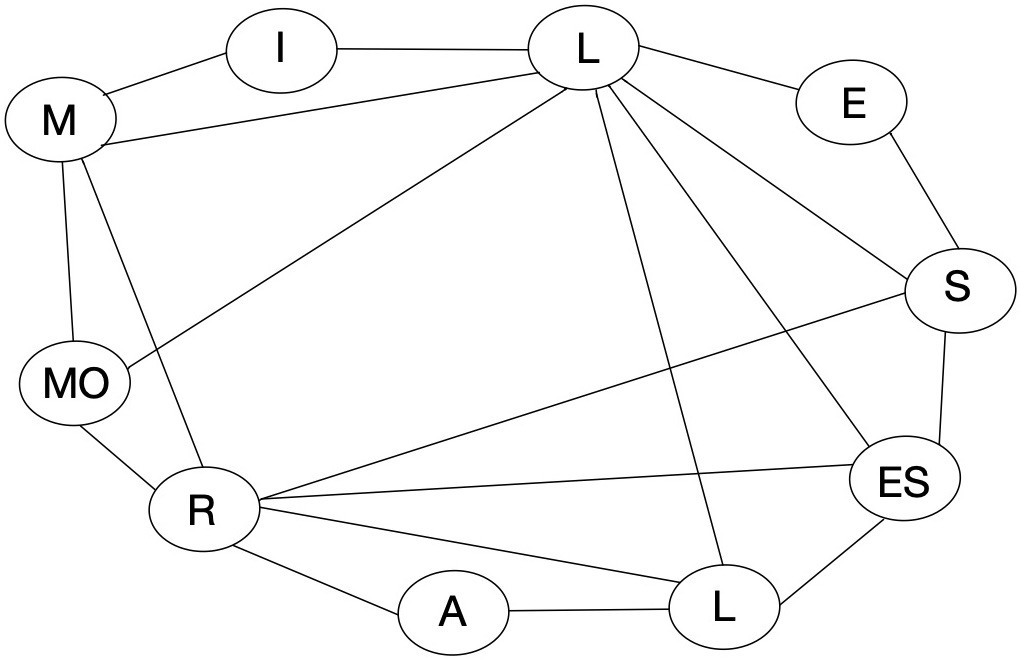
\includegraphics[width=13cm, height=6cm]{professors}
	\label{fig:professors}
\end{figure}


As networks increase in size, the possible shapes, and their implications, grow in complexity and potential value. Figure \ref{fig:professors} shows an example. In a social network of ten Reed computer science community members, there are a lot of questions to be asked. If I told you the student to professor ratio was 8:2, could you pick out who the two professors are without peeking at their long list of academic degrees? Instead, you can make observations based on their relation to the rest of the crowd. 

After a look at the network, one would notice that two of the people have a lot more connections than the rest. It's a safe assumption that the two professors are the people with the higher number of connections because students are interested in their wisdom, humor, and pictures of Eitan flying his plane! Similarly, what if I asked you to identify the tutor in a group of five Reed students (Figure \ref{fig:tutor}). It can be observed that there is only one person connected to every other. It would be a safe bet to say that the person in the middle is the tutor.

% pictures all use this same setup
\begin{figure}[h]
	\caption{Spot the tutor?}
	\centering
	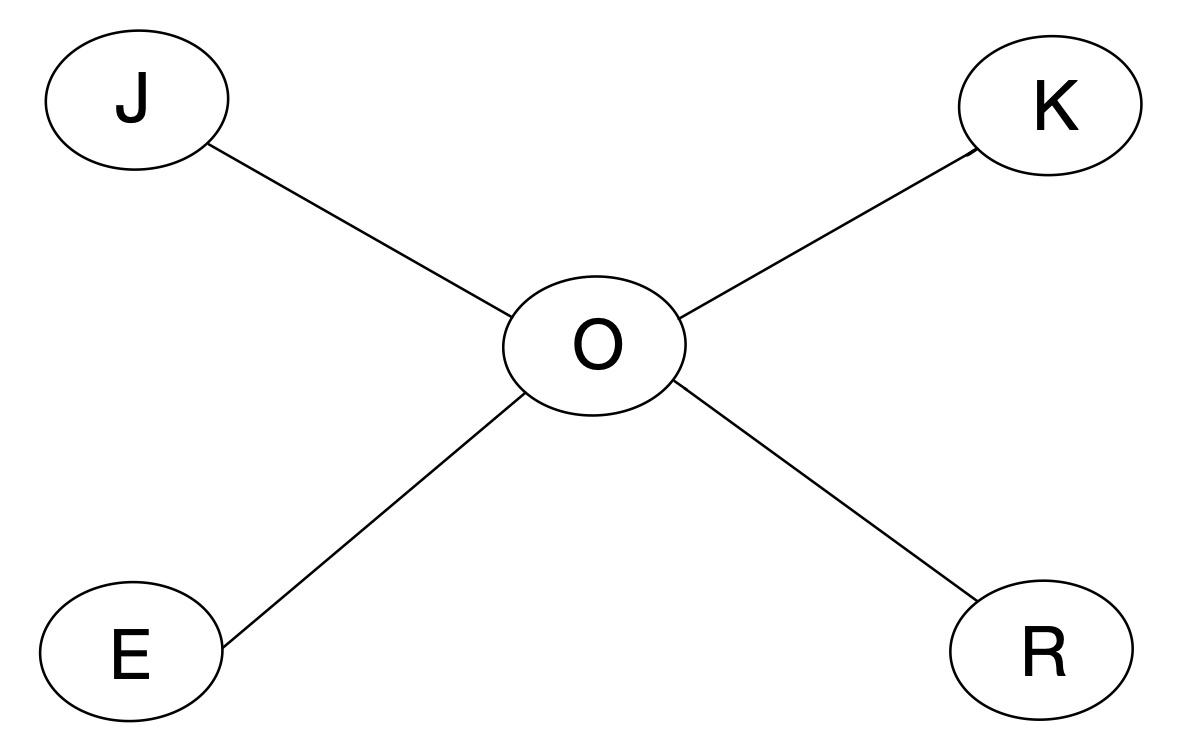
\includegraphics[width=5cm, height=3cm]{tutor}
	\label{fig:tutor}
\end{figure}

\section{Subgraph Counting}
Analysis of connections within a large network can be simplified with a bottom-up approach. Tens of millions of people in the US alone use Facebook on a daily basis. How can you analyze millions of people and the billions of connections between them? You break the larger problem into a smaller problem.

In a network of five people, you can focus on a smaller network of three people. The network of three people is a \textit{subgraph} of the original network. We will provide a more formal definition for subgraph in the next chapter. For now it is sufficient to think of a subgraph as a portion of a larger network. The focus of this thesis is tackling the \textit{subgraph counting problem} which can be defined as: given a specific collection of small graphs (triangles, squares, stars, etc...) and a network, how many times does each small graph occur as a subgraph within the larger network? In any network, there are certain patterns that are bound to become recurring characters. \textit{Network motifs} are reoccurring subgraphs whose regular occurrence or absence are of statistical significance. The motifs of interest vary depending on the application of this problem. So far we've seen an example of a star. Let's take a look at some other shapes that can occur in a network.

% pictures all use this same setup
\begin{figure}[h]
	\caption{Subgraph Counting}
	\centering
	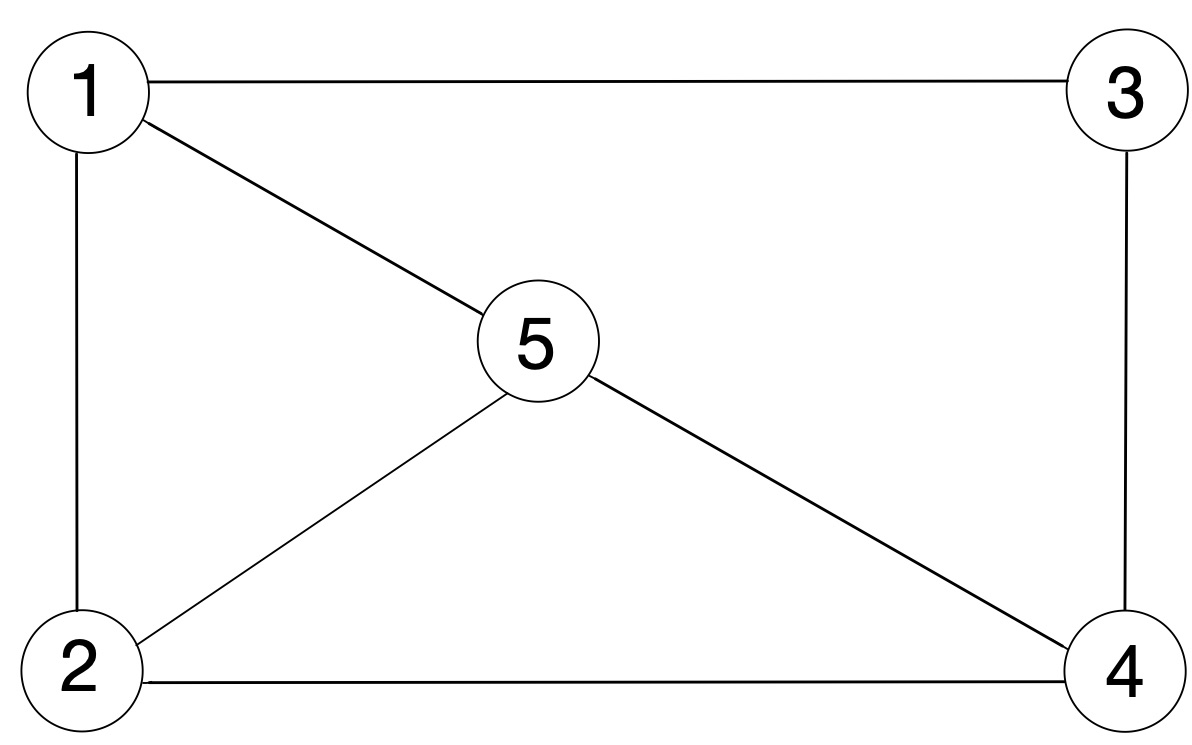
\includegraphics[width=6cm, height=4cm]{subgraphs}
	\label{fig:subgraphs}
\end{figure}

\begin{figure}[h]
	\caption{Subgraph Counts}
	\centering
	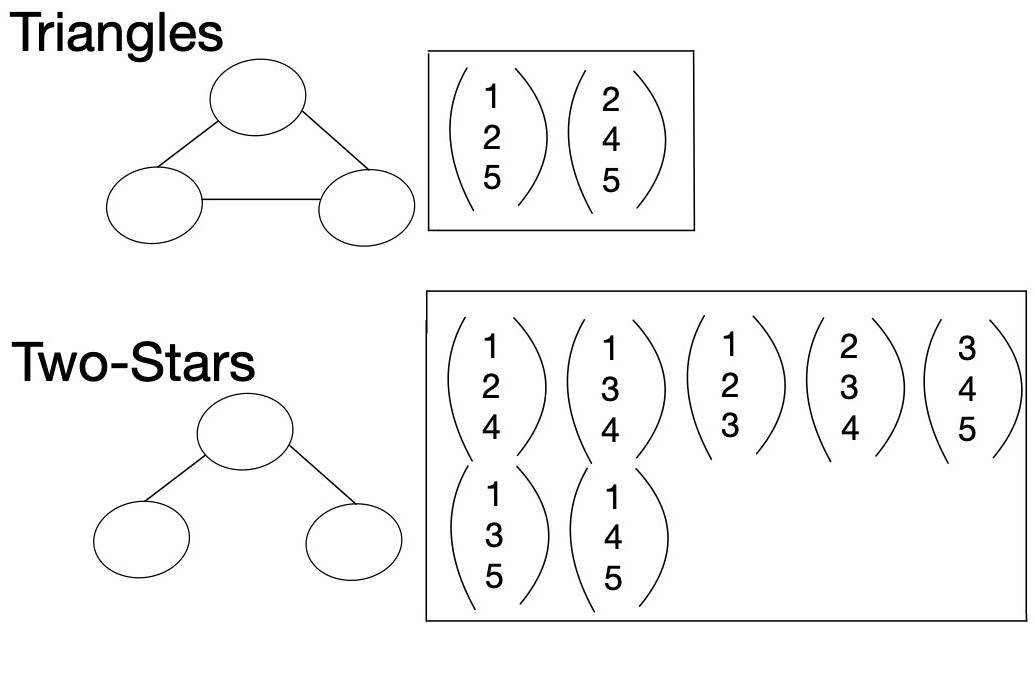
\includegraphics[width=6cm, height=4cm]{subgraph_motifs}
	\label{fig:subgraph_counts}
\end{figure}

Figures \ref{fig:subgraphs} and \ref{fig:subgraph_counts} give an example of subgraph counting within a larger network. Figure \ref{fig:subgraphs} shows a network with five participants and a total of seven connections between them. For this example, let's focus on two shapes of size three: triangles and two-stars. A triangle involves three participants with each one being connected to the other two. A two-star is the same with one less connection. Figure \ref{fig:subgraph_counts} shows the unique occurrences of these shapes in the larger graph. Something you may have noticed is that a two-star occurs within a triangle, but the participants within triangle are not counted as a two-star. This is because a motif occurrence must respect all connections (or lack thereof) of that specific shape. This is very relevant in the proper counting of shapes as we discuss in subsequent few chapters. It should also be noted that a single vertex can participate in different subgraphs as long as at least one vertex or edge is different. For example, 2 appears in two different triangles, $\{1,2,5\}$ and $\{2,4,5\}$.
	

\section{Trie Search}

% pictures all use this same setup
\begin{figure}[h]
	\caption{Prefix Trie Example}
	\centering
	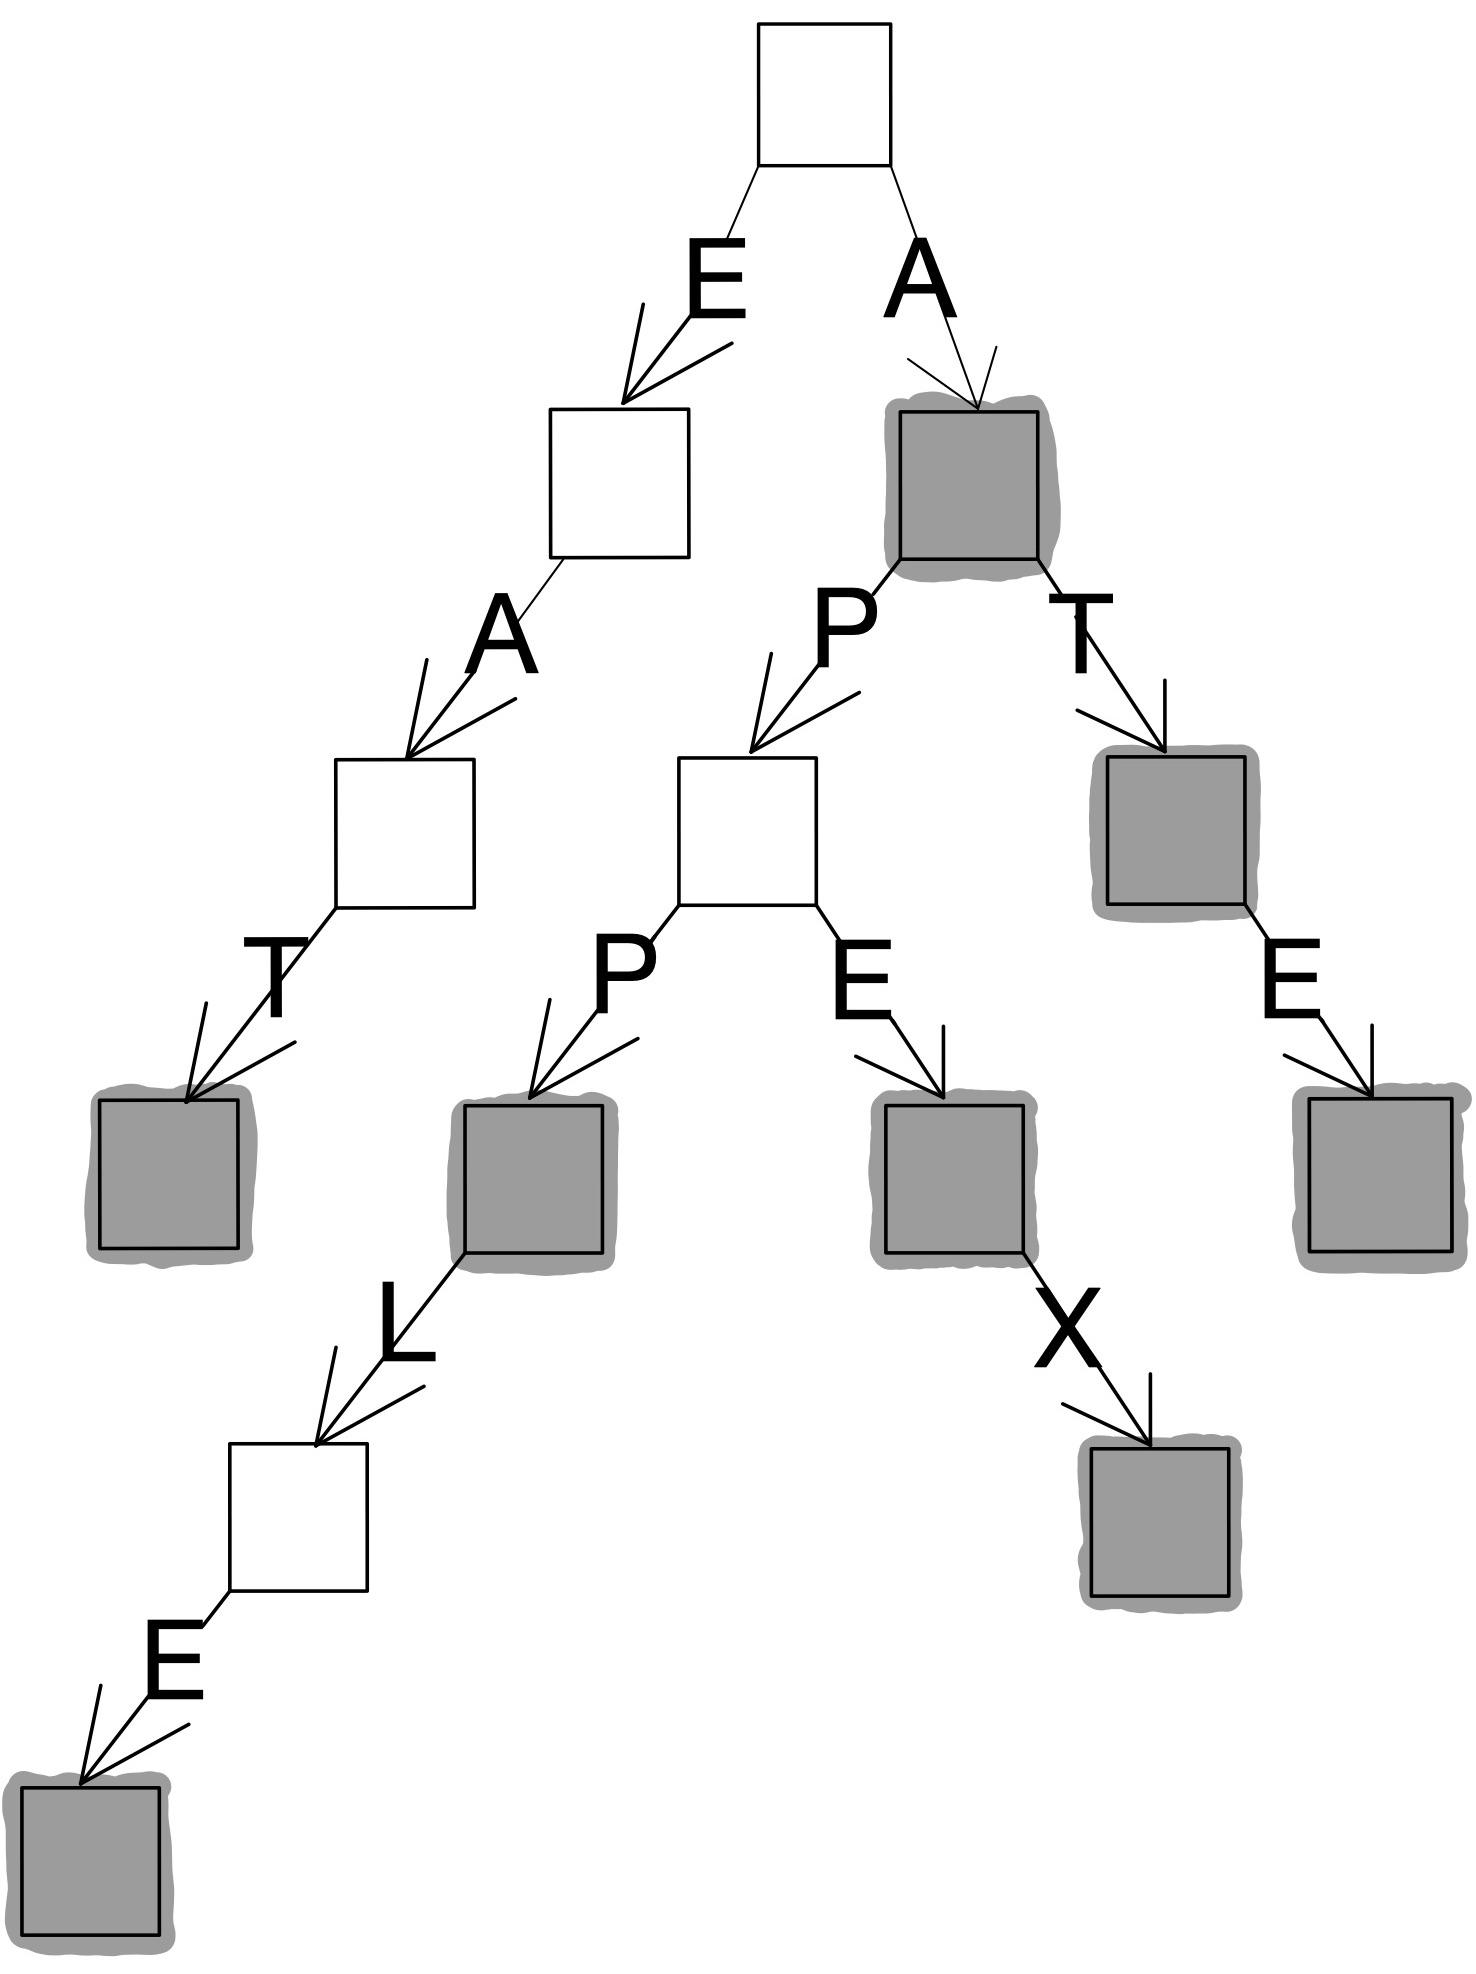
\includegraphics[width=4cm, height=5cm]{trie}
	\label{fig:trie}
\end{figure}

The primary structure we will be working with in this thesis is known as a graphlet trie (g-trie). Before defining a g-trie, let's use a similar structure known as a \textit{prefix trie} to build some intuition for how g-tries work.

Prefix tries are used to count how many times specific words occur in a text. A prefix trie organizes the text strings as a hierarchy organized as a parent/child relationship in a tree. The siblings within that tree all share the same prefix with their parent and ancestor strings. This structure gives us a compressed guide to the strings we are searching for in a long string of text. The empty string lives at the root of the tree, at each subsequent level, another letter is added to the current word path. A popular tradition at Reed is for seniors to insert random words in their thesis. Part of the fun is to "sneak" it past your adviser. If the adviser sees the sentence "Ape Ate: The gorilla game app whose apex includes guiding a gorilla to eat an apple," in the middle of a computer science thesis, they may grow suspicious. Conveniently, they can construct a trie similar to Figure \ref{fig:trie}  to see exactly how many times these words occur in the whole thesis. 

For example, let's look at the string "Ape Ate: The gorilla game app whose apex includes guiding a gorilla to eat an apple." Scanning through, we start with the word "ape." The letter "a" is scanned first, so we take one step down the right side of the tree. Next is "p" so we step down and left, followed by "e" with a step right. Now that we are at the end of the word, we notice that the box after the final letter is highlighted, indicating that it is a word of interest. Because of this, we increase the count of occurrences for the word "ape." If we were just scanning the word "ap", we would not count it because it is not a word of interest (or an english word at all). Given the context, it is unlikely that the adviser would see many occurrences of most of these words. They can use this low count to make an informed guess that this sentence has ulterior motives.

The benefits of this approach start with having the ability to search for common or related strings in a larger text. Once you find them, the trie offers a convenient and space-efficient way to store them. Let's say someone took this same trie and applied it to a biology textbook. One would reasonably expect this to result in words appearing more frequently. With that increased frequency, we get the benefit of compression. Using a trie relieves the need to store each occurrence of a word. Instead we can follow the path to that work and only store relevant information at the node. This can include location of the word or just an incremented counter. It can also be helpful to have a means for comparing the occurrences of words with a similar ancestry. An example of this is using tries to check the usage of words with various spellings (grey vs gray, enrol vs enroll, lambaste vs lambast, etc...).
%currently, g-trie is getting defined twice?

That being said, this thesis considers graph search instead of text search. In doing so, we work to find occurrences of \textit{graphlets}, small subgraphs within a larger network. To differentiate between motifs and graphlets, think back to figure \ref{fig:subgraphs}. A triangle is considered a motif, while the specific occurrence of $\{1,2,5\}$ is a graphlet. Graphlet search is the network analogue to text search. We explore use of a g-trie data structure. This is the network analogue to a prefix trie. It is used to guide the algorithms of our network search. Figure \ref{fig:motifs} characterizes the g-trie we use in chapters 3 and 4.

% pictures all use this same setup
\begin{figure}[h]
	\centering
	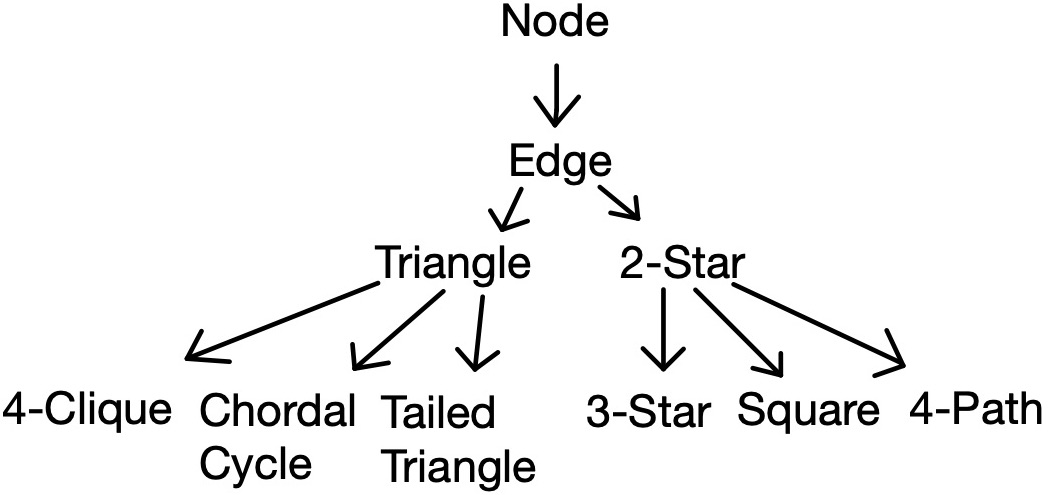
\includegraphics[width=5cm, height=4.5cm]{motifs_names}
	\caption{Network Motifs}
	\label{fig:motifs}
\end{figure}

Like the prefix trie, it is a tree where nodes corresponds to items we seek in our search. Rather than being short text strings like "Eat", these are instead small graphs like the triangle, star, or two-star. Figure \ref{fig:motifs} shows ten nodes that represent the possible combinations of one, two, three, and four vertices within a graph. Similar to the prefix trie, there is a parent-child relationship encoded by the tree. Since a four-clique of four vertices, contains a triangle of three vertices, it sits below the triangle in the g-trie.

G-tries are very similar to prefix tries. Each step you take adds a vertex to a graph path, and has a similar mechanism that highlights the trie nodes of interest. This is depicted in Figure \ref{fig:motif_shapes}, showing the behind the scenes representation of Figure \ref{fig:motifs}. For the purposes of my research, all motifs of size three and size four will be deemed nodes of interest. Large scale subgraph counting becomes much slower when computing subgraphs of size four or greater. Because of this, focusing on "easy" subgraphs of size three and harder subgraphs of size four has shown to be a balanced approach that is scalable to subgraphs of size $n$. For $n > 4$ the tree would continue to grow to $n$ levels.

%"under the hood this is whats happening"
\begin{figure}[h]
	\caption{Motif Shapes}
	\centering
	\resizebox{10cm}{!}{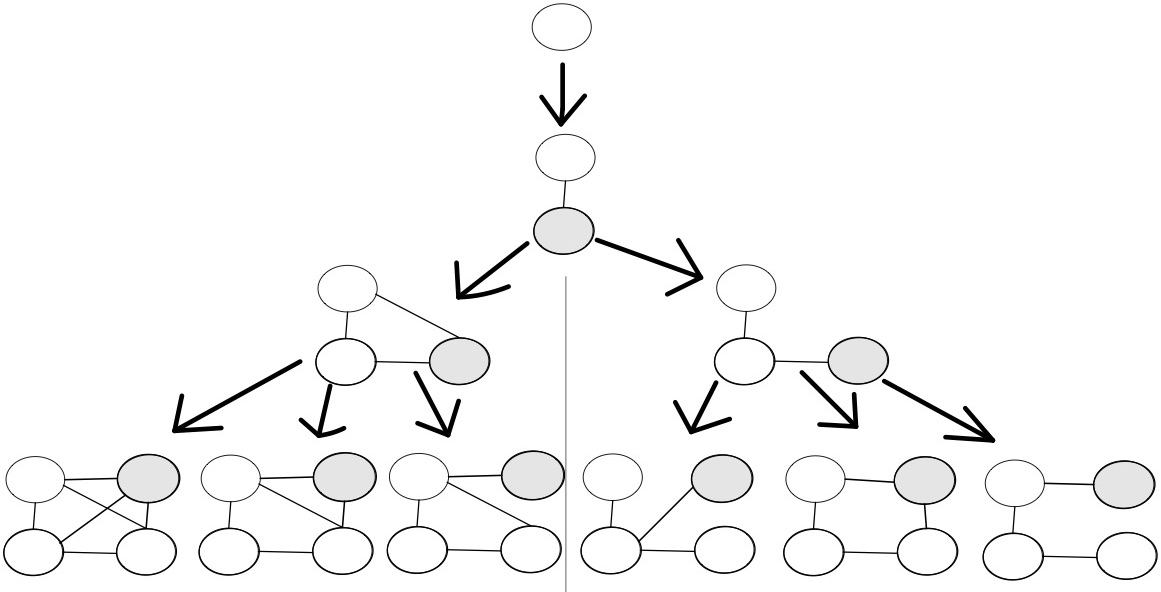
\includegraphics{motifs_shapes}}
	%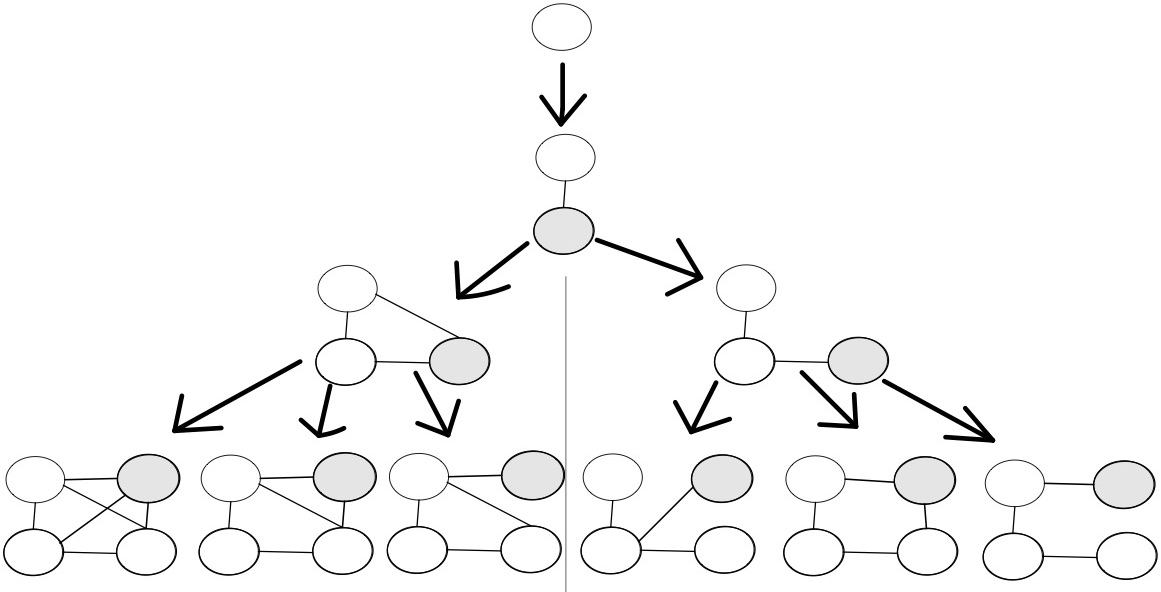
\includegraphics[width=8cm, height=7.5cm]{motifs_shapes}
	\label{fig:motif_shapes}
\end{figure}


%-Talk about value of shapes (and applications within real world networks)
\section{Graphlet Census in Computational Biology}

%Will want to do a better job putting this in my own words, can probably ask Jim how worried I should be about plaigurism here
In the field of computational biology, there exist many use cases for analyzing the topology of a network. Different types of cellular networks are frequently represented as a graph (see \citeauthor{bio_graphlets} \cite{bio_graphlets} for an example). Vertices represent biological components such as proteins or genes. The physical and/or chemical interactions between them are represented as edges. This analysis extends to local and global topologies within a network. Graphlet census is often helpful for focusing on local structures, but has applications on both levels. Protein-protein interaction (PPI) networks, cell signaling networks, and metabolism networks are all examples of networks that have a history of meaningful research using graphlets. This history includes the comparison of diseased and healthy cell networks to inform treatment plans; as well as cross-species comparisons that allow for insights into evolutionary progress. Brain networks \cite{bio_brain}, disease genes \cite{bio_disease}, and PPI networks \cite{bio_graphlets} have all benefited from research using graphlets. Most cases use motifs up to size five. Graphlet research in this field is limited by graphlets being better suited for undirected graphs. For certain biological use cases, the directionality of an edge holds a lot of valuable information that does not translate well to an undirected search. That being said, it is possible to alter the common approach to fit the needs of a directed graph.
%but I encourage you to look into \cite{bio_graphlets} to learn more about approaches that fit this specific need.

As we grow older, humans become more susceptible to disease. Graphlet census has been useful in research focusing on how the aging of cells contributes to this. GDD analysis allowed Faisal and Milenkovic \cite{bio_aging} to draw conclusions about global and local topologies of different PPI networks. They compared networks known to be related to aging with those they predicted to also be aging related. This relation worked in conjunction with analysis into the overlap between the two network sets in terms of their involvement in aging-related, and non-aging related diseases. That being said, graphlets were able to serve their work beyond the use cases in this thesis. In the process of performing a graphlet census, they also stored how many graphlets a particular vertex participated in. This allowed them to measure a specific vertex's centrality. Vertices with a higher level of connectedness serve as an excellent opportunity for treatment. Drugs targeting well connected proteins allow for a treatment with higher impact (as opposed to targeting proteins in more sparse areas of the network).

%\textbf{Disease}
\citeauthor{bio_disease} \cite{bio_disease} used various methods of comparing disease networks. Graphlets were the only method based on network topology. Specifically, they conducted a graphlet census to compare genes in human PPI networks. In addition to that, graphlets were used to compare diseases and gain a further understanding of the reason behind and likelihood of co-occurrence for a given pair of diseases. This type of research allows for an increased understanding in how diseases spread and the conditions in which they thrive. It also helps differentiate between diseases with overlapping symptoms. Similar work has also shown this to be useful in disease treatment. In cases where one is trying to treat a lesser-known disease, it helps to classify it accurately among better understood diseases.

%\textbf{Brain}
Graphlets can also be used for brain research. Brain networks have been identified as "small world" networks \cite{bio_graphlets}. This means that any neuron (vertex) is only a few connections away from any other neuron in the network. Interestingly enough, there have been studies showing neural path lengths have an inverse relationship with a person's IQ. This shows that the "small world" structure of neural networks is directly tied to its efficiency. \citeauthor{bio_brain} looked at a subsection of these networks known as brain functional networks (BFN). While a lot of brain function can be recorded non-invasively using electroencephalography (EEG), BFN requires the higher level of precision granted by invasive procedures using electroencephalography (ECoG). BFN are in charge of working together to respond to changing stimuli and performing cognitive functions. \citeauthor{bio_brain} \cite{bio_brain} used Graphlet Degree Distribution to compare the structure of the brain as it performed various tasks. This collection of motif counts serves as the fingerprint for a network, allowing it to be compared to other networks. This study focused on comparing neural activity for one person across different tasks, and across different people on similar tasks.

%\subsection{anonymous networks}





% Double spacing: if you want to double space, or one and a half 
% space, uncomment one of the following lines. You can go back to 
% single spacing with the \singlespacing command.
% \onehalfspacing
% \doublespacing

		\chapter{Preliminaries}

\section{Graphs}

%(maybe include induced subgraph for good context) {reference Jiarong's section 2.0.4 for guidance)	
In mathematics, the abstract object most often used to represent networks is called a \textbf{graph}. This models the relationship between a collection of entities represented by vertices, and the connections among them, represented by the graph's edges.

\begin{definition} [Graph]
\label{def:graph}
A graph $G = (V,E)$ consists of a set of \textbf{vertices} $V$ and a set of \textbf{edges} $E$ $\{ (u,v)  \ | \ u,v \in V, u \neq v\}$

\end{definition}

\begin{definition} [Graph Types]
\label{def:graph_types}
A graph $G$ is \textit{directed} when all $e \in E(G)$ are interpreted as ordered pairs. $G$ is undirected when they are interpreted as unordered pairs, that is, subsets of size 2.
\end{definition}

Given a formal definition, we can represent the graph in Figure \ref{fig:tutor} as $G = (\{E,J,K,O,R\}, \{(E,O), (J,O), (K,O), (R,O)\})$. Thus far, we have only been depicting undirected graphs. $J$ knows $O$ so there exists an edge $(O,J)$. This is the same as the edge $(J,O)$. If instead, we were depicting the "$X$ consulted $Y$" relationship of tutoring, then we would have a directed graph where all edges point to the tutor $O$. This would give us the edge set $\{ (J,O), (K,O), (E,O),(R,O) \}$. The return edges (such as $(O,J)$ would not exist unless the tutor consulted one of her tutees.

Weighted graphs are common in travel networks. The weight of an edge is often associated with the time or cost of a given route. Weights are also used behind the scenes to represent the strength of connections in social networks. People who interact more frequently or have more in common, have a higher weight than those with less interaction. Figure \ref{fig:social_triangle} shows a small example of a weighted social graph.

\begin{figure}[h]
	\centering
	\caption{Weighted Social Triangle }
	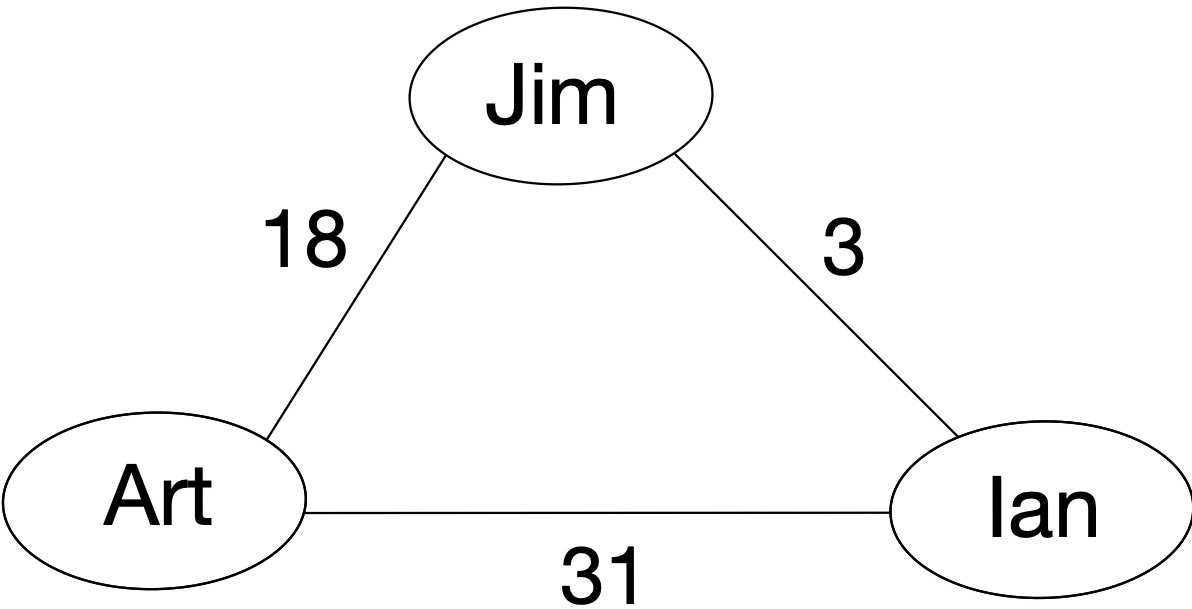
\includegraphics[width=6cm, height=4cm]{social_triangle}
	\label{fig:social_triangle} %walk_3 is just showing that we crossed out the one we have already processed
\end{figure}

In Figure \ref{fig:social_triangle}, Art, Jim, and Ian are all friends with varying weights between them. Art and Jim meet weekly and keep a consistent rapport, so they have built up a weight of 18. Art and Ian live together so they have a higher weight of 31. Jim and Ian have not spoke much since Ian's graduation, so their weight is only a 3. Figure \ref{fig:dir_undir} depicts an example of directed versus undirected graphs. The directionality of edges is similar to social media structures. The way Twitter handles interpersonal connections is similar to a directed graph. Just because I follow LeBron James, does not mean he follows me back. Undirected graphs are more akin to Facebook friends: I can only "friend" with Jim if and only if he is willing to "friend" me. 

\begin{figure}[h]
	\centering
	\caption{Directed vs Undirected Edges}
	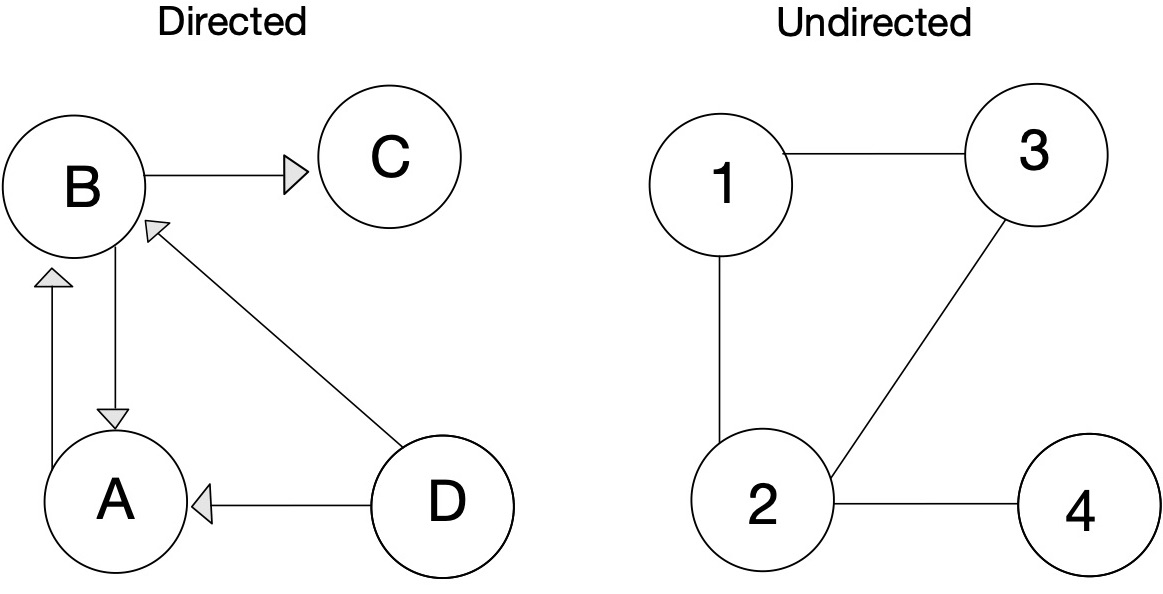
\includegraphics[width=5cm, height=3cm]{directed_undirected}
	\label{fig:dir_undir} %walk_3 is just showing that we crossed out the one we have already processed
\end{figure}


\begin{definition} [Neighbor and Degree]
\label{def:neighbor_degree}
For vertices $v, u \in V(G), v$ is a neighbor of $u$ if and only if $(u,v) \in E(G)$. The set of neighbors of vertex $v$ is denoted $N(v)$. The degree of $v$ is $ | N(v)|$.
\end{definition}

In social networks, friends are equivalent to neighbors. The number of friends someone has is their degree. For directed graphs, there are \textit{indegree} and \textit{outdegree}. Indegree counts the number of incoming edges (number of followers), while outdegree counts the number of outgoing edges (number of people you follow).

With rows and columns indexed by $V(G)$, the \textbf{adjacency matrix} of $G$ is another representation of its connections. If $A$ is an adjacency matrix, then $A[u,v]$ has the entry $1$ whenever $(u,v) \in E(G)$ and is $0$ otherwise. For undirected graphs, this is a diagonally symmetrical matrix. The following matrix is the adjacency matrix for the undirected graph in Figure \ref{fig:dir_undir}.

\[
\begin{blockarray}{ccccc}
1&2&3&4 \\
\begin{block}{(cccc)c}
0&1&1&0&1 \\
1&0&1&1&2 \\
1&1&0&0&3 \\
0&1&0&0&4 \\
\end{block}
\end{blockarray}
 \]

\begin{definition} [Subgraph]
\label{def:subgraph}
A graph $G'$ is a subgraph of graph $G$ whenever $V(G') \subseteq V(G)$ and $E(G') \subseteq E(G)$. We denote the set of subgraphs of $G$ as $S(G)$.
\end{definition}

\begin{definition} [Induced Subgraph]
\label{def:induced_subgraph}
Let $G = (V,E)$ and $V' \subseteq V$. The subgraph induced by $V'$ is the graph $G' = (V',E')$ where $E' = \{(u,v) \in E \ | \ u,v \in V' \}$
\end{definition}

An induced subgraph is a subset of vertices of graph $G$ along with any edges whose endpoints are both in the subset. Figure \ref{fig:ind_sub} depicts a graph $G_{1}$, and two subgraphs, $G_{2}$ and  $G_{3}$. Both subgraphs are over the vertex set $\{1,4,5 \}$. $G_{2}$ is an induced subgraph, while $G_{3}$ is not because it is missing the edge $(4,5)$. 

\begin{figure}[h]
	\centering
	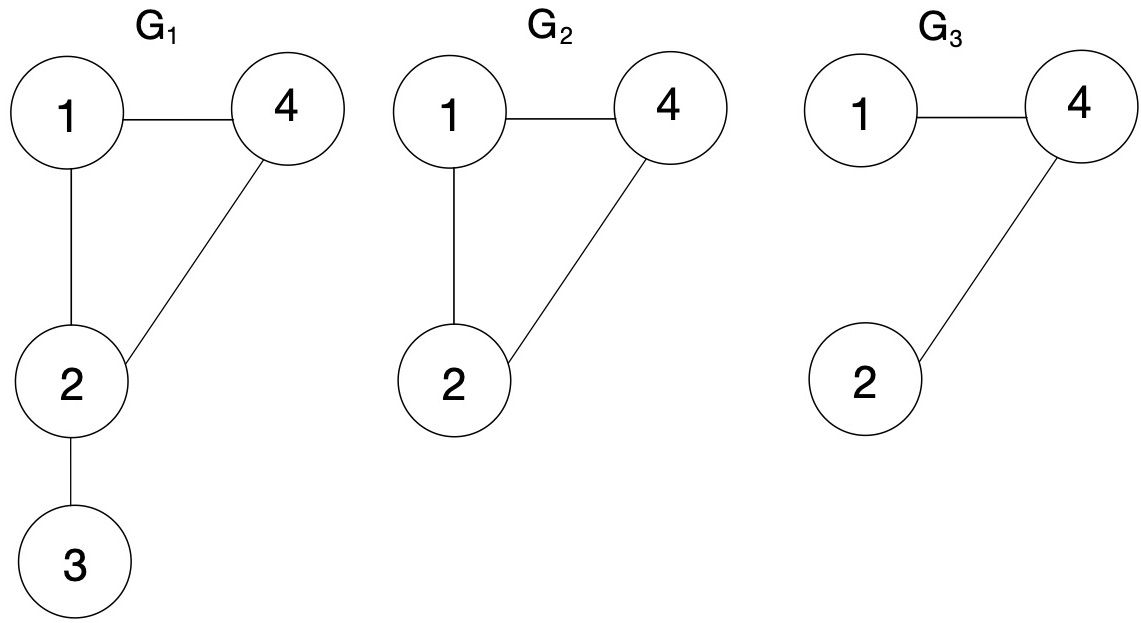
\includegraphics[width=6cm, height=3cm]{ind_sub}
	\caption[Induced Subgraphs]{G$_2$ and G$_3$ are subgraphs of G$_1$. G$_2$ is induced by $\{1,2,3\}$ and G$_3$ is not.}
	\label{fig:ind_sub}
\end{figure}


%Do we want to say something about
\begin{definition} [Graph Restriction]
\label{def:restriction}
Let $X \subseteq V(G)$. We denote the subgraph induced by $X$ as $G/X$.
\end{definition}

\section{Graph Isomorphism}

\begin{definition} [Isomorphism]
\label{def:isomorphism}
An isomorphism of graphs $G$ and $H$ is a bijection $f : V(G) \to V(H)$ such that $(u,v) \in E(G)$ if and only if $(f(u), f(v)) \in E(H)$. When G is isomorphic to H, we write $G \sim H$.
\end{definition}

\begin{figure}[h]
	\centering
	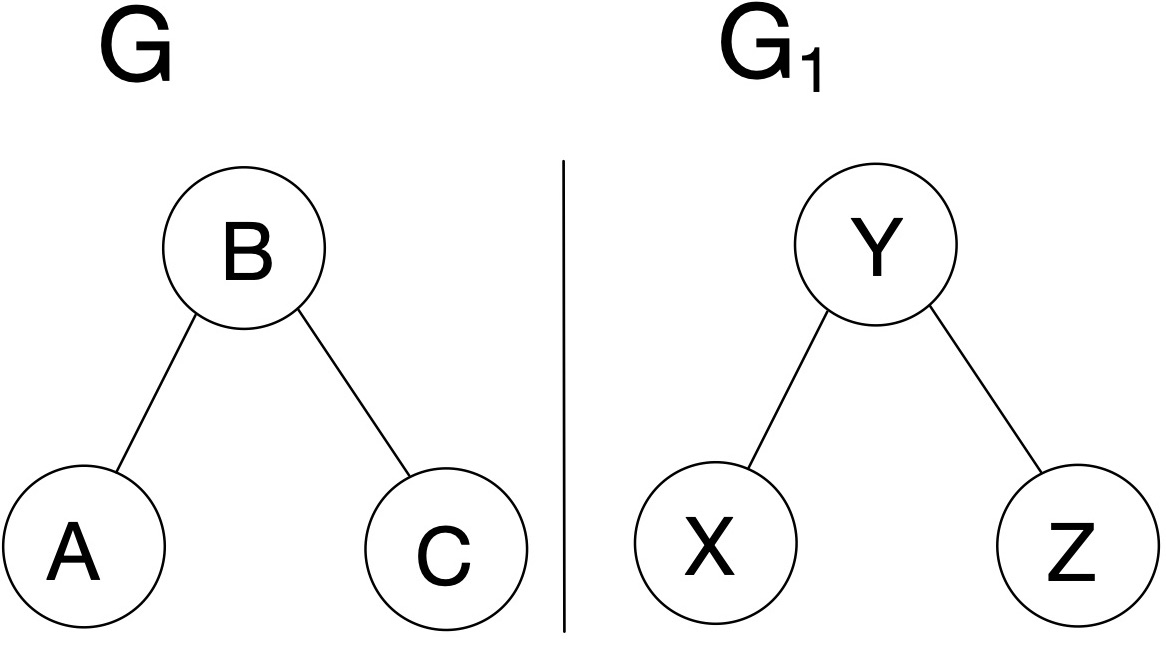
\includegraphics[width=4cm, height=2cm]{iso_1}
	\caption{Isomorphism Ex. 1}
	\label{fig:iso_1}
\end{figure}

\begin{figure}[h]
	\centering
	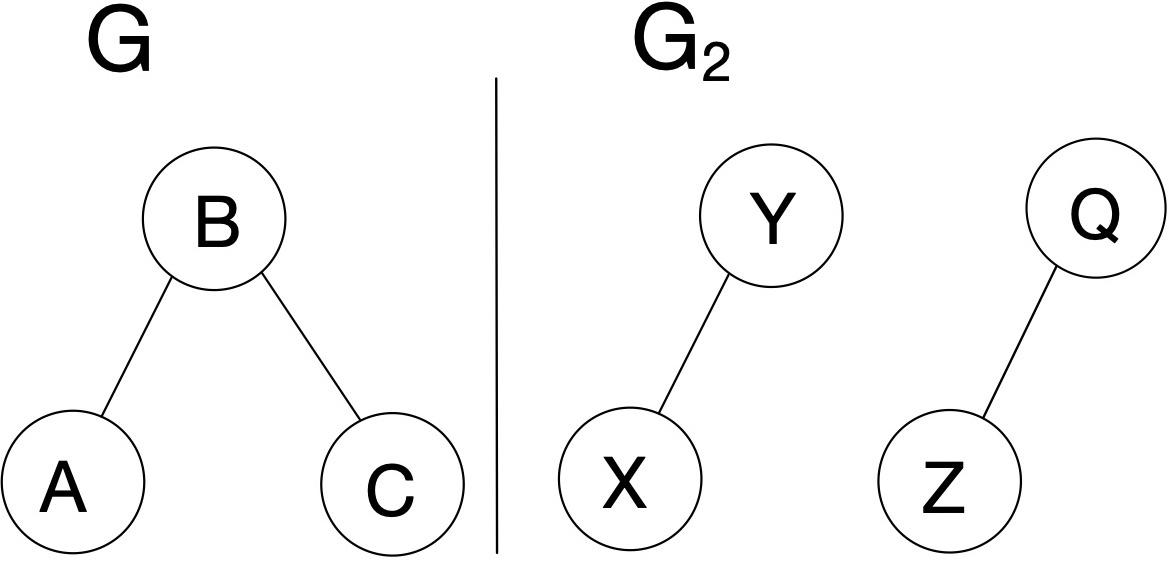
\includegraphics[width=4cm, height=2cm]{not_iso_2}
	\caption{Isomorphism Ex. 2}
	\label{fig:iso_2}
\end{figure}

\begin{figure}[h]
	\centering
	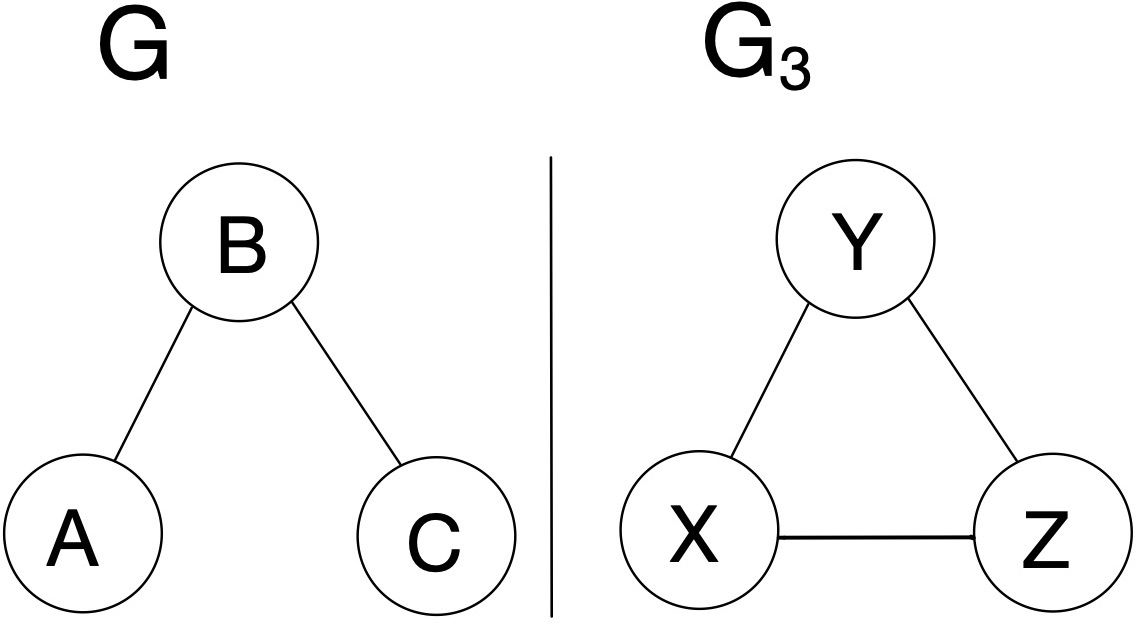
\includegraphics[width=4cm, height=2cm]{not_iso_3}
	\caption{Isomorphism Ex. 3}
	\label{fig:iso_3}
\end{figure}

Two graphs $G$ and $H$ are isomorphic when there is a correspondence between their vertices that preserves connectivity. If no correspondence exists where the connections of $H$ respect the connections of $G$, then they are not isomorphic, i.e. $G \nsim H$. Let's look at some small examples to develop some intuition. Let:

\begin{itemize}
		\item $G = (\{A,B,C\}, \{(A,B), (B,C)\})$
		\item $G_{1} = (\{X,Y,Z\}, \{(X,Z), (Y,X)\})$
		\item $G_{2} = (\{X,Y,Z,Q\}, \{(X,Y), (Q,Z)\})$
		\item $G_{3} = (\{X,Y,Z\}, \{(X,Z), (Y,X), (Y,Z)\})$
\end{itemize}

Intuitively, $G \sim G_{1}$ because $|E(G)| = |E(G_{1})|, |V(G)| = |V(G_{1})|,$ and the edge structure of $G$ can be preserved by $G_{1}$ (Figure \ref{fig:iso_1}). $G \nsim G_{2}$ because $|V(G)| < |V(G_{2})|$ (Figure \ref{fig:iso_2}). It follows that $G \nsim G_{3}$ because $|E(G)| < |E(G_{3})|$ (Figure \ref{fig:iso_3}). Now that we have a sense for induced subgraphs, let's take a closer look at what a graphlet is. In the literature, a \textit{graphlet} is any of the collections of undirected graphs of some size $k$, where $k$ is typically small. For example, \citeauthor{g_tries} \cite{g_tries} considered graphlets with up to 4 vertices, so $k = 4$. In Figure \ref{fig:motifs}, we see subgraphs corresponding to graphlets of size one, two, three, and four. A graphlet $g$ occurs in a graph $G$ when there is a set of vertices $X \subseteq V(G)$ s.t.  $G/X \sim g$. For example, in Figure \ref{fig:simple_census}, there are two triangle occurrences. The larger graph restricted to the vertex set $\{S,B,C\}$, is isomorphic to the shape of a triangle.

%Not really sure what Jim was talking about here
%\begin{figure}[h]
%	\centering
%	\resizebox{5cm}{!}{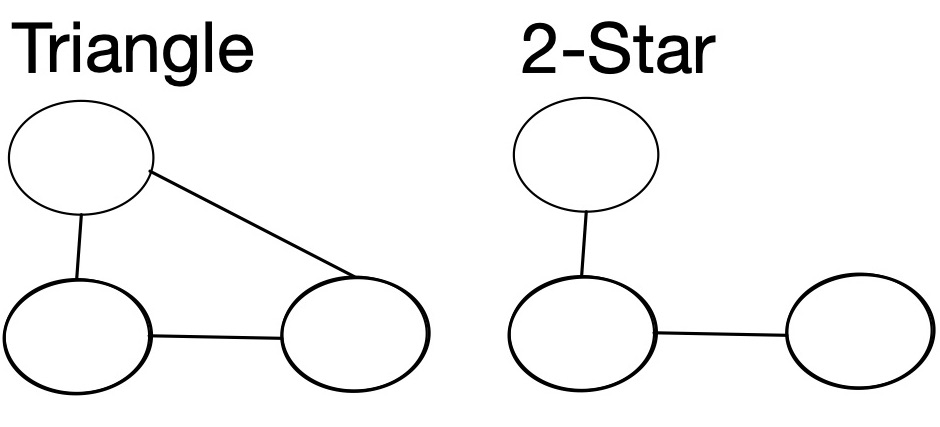
\includegraphics{motif_three}}
%	\caption{Motifs of size three}
%	\label{fig:motifs_three}
%\end{figure}

\subsection{Complexity of Finding Isomorphisms}

The \textit{subgraph isomorphism problem} can be stated as: given graphs $\{G, G', H \ | \  G' \in S(G) \}$, determine if $H \sim G'$. This problem is well known to be \textit{NP-complete}. NP is a class of decision problems\footnote{A decision problem has a yes or no answer} for which there exists a polynomial-time\footnote{Polynomial time is defined as: $O(n^c)$ or better where $c$ is a constant value} verifier for possible solutions. NP-complete problems are ones that, by a very technical definition that we omit here, are the hardest problems in the class NP. These hard problems are not believed to have any efficient algorithm for solving them. A problem related to our problems of study is the \textit{clique} problem. A $k$-clique is a subgraph of size $k$ where all vertices in that subgraph are connected by edges. For example, a triangle is a 3-clique. Determining whether a graph has a clique of size $k$ is NP-complete. The graph isomorphism problem---the algorithmic question as to whether two graphs are isomorphic---is also believed to be a computationally hard problem. It is not known to be NP-complete, yet it is believed to be computationally hard to solve. Some algorithmic complexity researchers believe it to be neither in P nor NP-complete. Of course, for this to be resolved we would need to know whether P $\neq$ NP.

\section{Graphlet Census} \label{sec:sub_cens}

The focus of this thesis is to find sequential and parallel solutions to the \textit{subgraph counting problem}. These subgraph occurrences within a larger graph are known as graphlets.  The \textit{Graphlet Degree Distribution} (or  {GDD}) is the table used to keep track of these motifs. Each time a new occurrence of motif \textit{m} is found, GDD[\textit{m}] is incremented by one. When completed, the counts of all motifs serves as the network fingerprint.

\begin{figure}[h]
	\caption{Graphlet Census}
	\centering
	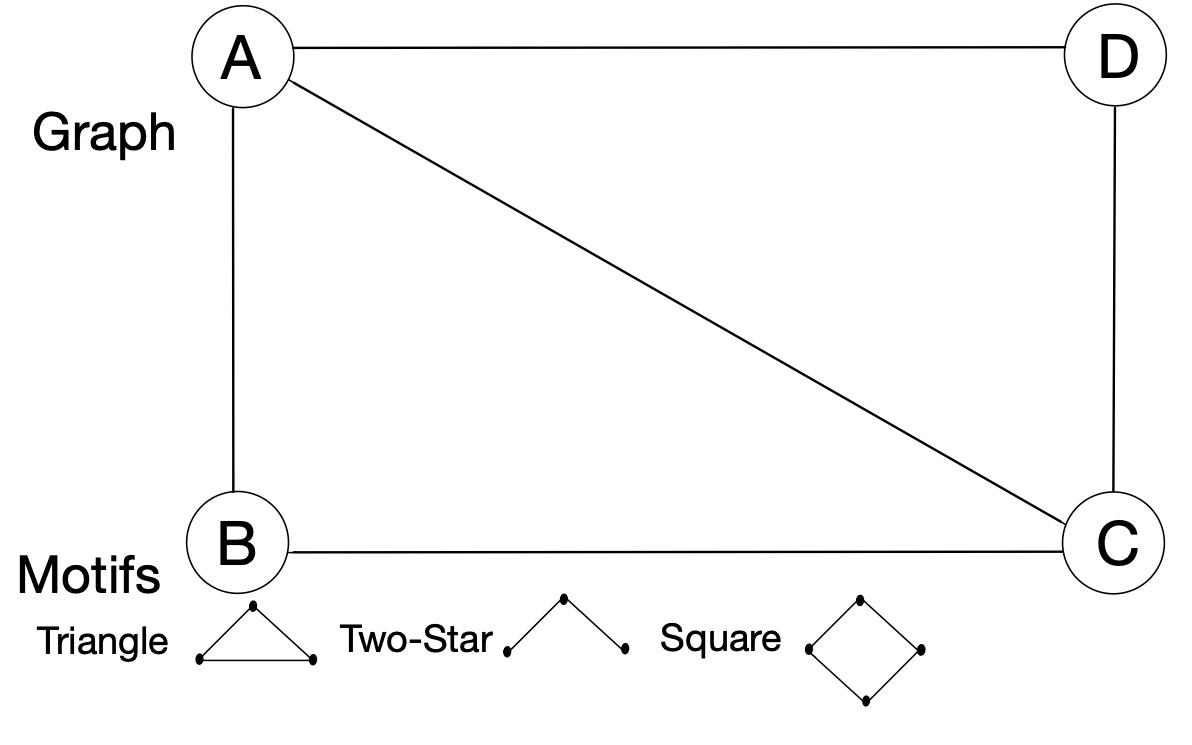
\includegraphics[width=6cm, height=4cm]{simple_census}
	\label{fig:simple_census}
\end{figure}

\begin{table}[h!]
\begin{tabular}{ |p{3cm}|p{3cm}|p{3cm}| }
	 \hline
 	\multicolumn{3}{|c|}{Graphlet Degree Distribution} \\
 	\hline
	Motif& Count &Graphlets\\
 	\hline
 	Triangle   & 2    &\{ABC\}, \{ACD\}\\
 	Two Star&   2  & \{BCD\}, \{BAD\}  \\
 	Square &1 &\{ABCD\}  \\
	 \hline
\end{tabular}
 \caption{Simple Census Table}
\label{table:simple_census}
\end{table}

	\subsection{Example}
Table \ref{table:simple_census} shows the GDD for Figure \ref{fig:simple_census}. This census counts triangles, two stars, and squares. It is important to note, that one motif may occur within another of the same degree. Every triangle includes a two star, but it isn't counted as a two star because that collection of vertices has the additional edge a two star is missing. In our algorithm, the motif's adjacency matrix is what helps separate this. The final vertex in a triangle would have a $\{1,1\}$ relationship to the previous two. This means a connection does exist between the last vertex and each of the first two.This contrasts with the final vertex of a two star having a $\{0,1\}$ relationship, meaning the latest vertex does not share an edge with the first one.

\subsection{Complexity of Subgraph Counting}
The subgraph counting problem is computationally hard. If it is hard to compute whether or not a subgraph occurs within a network, it follows that counting all occurrences of multiple subgraphs is even harder. As the motifs of interest increase in size, the overall runtime also grows. Parallelization and g-tries are tools that allow us to work faster and limit the exhaustive search for graphlets. The next section provides additional information to help establish the usefulness of these techniques.
	
\subsection{Naive Approach}
A naive algorithm for the subgraph counting problem would do an individual search for each possible shape. Initial trials started with motifs of degree three. The following pseudocode shows a brute force solution to searching for all \textit{triangles} and \textit{two-stars} in a graph.

\begin{algorithm}
\caption{Brute force subgraph counting of size 3 in graph $G$}
\label{alg:naive}
\begin{algorithmic}[1]

\Function{SubgraphCounting}{$G$}
    \State $triangles = []$
    \State $twoStars = []$
    \For{ $v_1 \in V(G)$} 
    \For{ $v_2 \in N(v_1)$} 
    \For{ $v_3 \in N(v_2)$}
    
    \If{$v_3 \in N(v_1)$}
        \State $triangles = triangles \cup \{v_1, v_2, v_3\}$
    
    \Else
         \State $twoStars = twoStars \cup \{v_1, v_2, v_3\}$
    \EndIf
    \EndFor
    \EndFor
    \EndFor
    \State \Return $triangles, twoStars$
    
\EndFunction

\end{algorithmic}
\end{algorithm}

Algorithm \ref{alg:naive} is constructed of a triply nested loop. The first of which scans through all graph vertices. The second loops through the neighbors of the current $v_1$ and the second loops through the neighbors of $v_2$. If there exists an edge $(v_1,v_3)$ then the shape is counted as a triangle (line 7), otherwise the shape is counted as a two star. This algorithm runs in $O(|V|^3)$ time.

This approach has a number of issues. The primary one being that every graphlet is found three times. For every triangle $\{1,2,3\}$, time would be wasted also finding $\{2,1,3\}, \{2,3,1\}$ and so on. As currently constructed, we would overcount graphlet occurrences.
%Can save this for later?
% A correct solution for this could sort the vertices in a graphlet and use a set object to avoid counting repeats.
	
Another issue with this approach is that there must be a completely new search for each shape. As we saw in Figure \ref{fig:motifs}, the motifs of degree three build on motifs of size two. Motifs of degree four build on motifs of degree three and so on. Every motif of degree four benefits from being calculated from its parent graphlet. In algorithm \ref{alg:naive} we are only searching for motifs of size three. We can do two in one search because there is only one edge that differentiates a \textit{triangle} from a \textit{two-star}. For motifs of size four and beyond, this is not as simple as singular if statement. Early in this process, I tinkered with the algorithm such that I combine multiple motifs of size four in one function. This idea still resulted in multiple scans over all $V \in G$ just for motifs of size four. Then you factor in having to do so again for size three, (and larger depending on the application) and things get messy and inefficient. 
	
For motifs of size three, the runtime is $O(|V|^3)$. It follows intuitively that for motifs of size four, it would grow to $O(|V|^4)$ and that is just for one motif! There are ways to optimize this search with techniques such as symmetry breaking conditions, but fundamentally, it does not scale well.  The next chapter introduces \textit{graphlet-tries}, which will be the next step in our quest for sequential success.

\section{What is Parallelization?} \label{sec:pre_para}
Imagine you and a friend are working on 100 Christmas cards split 50--50. When you are done, your friend has 10 cards remaining, so you split the last 10, 5--5. This way, you are not waiting while your friend works and the overall task gets done faster. The power of good teamwork translates well into the computational world, with some tasks benefiting greatly from a parallel "split the work" approach. 

\textit{Parallel algorithms} are ones where different processors are performing computations simultaneously to solve a problem. One way to do this is to decompose a problem into several smaller subproblems and have them processed and solved in parallel. To illustrate the idea, consider the problem of summing the numbers in an array.

\subsection{Example}
\begin{algorithm}
\caption{Sequential Array Sum}
\label{alg:seq_sum}
\begin{algorithmic}[1]

\Function {SequentialSum}{$A$}
    \State $sum = 0$
    \State $i = 0$
    \While{$i < A.size$}
    	\State $sum = sum + A[i]$
	\State $i = i + 1$
    \EndWhile
    \State \Return sum
\EndFunction

\end{algorithmic}
\end{algorithm}

Let an array $A$ be comprised of $n$ numbers that need to be added together with $A[i]$ denoting the $i^{th}$ element of $A$. An initial attempt to solve this problem would scan the array and track a running total that is modified with each element processed (Algorithm \ref{alg:seq_sum}). One processor can add up the values of $A$ in $\Theta (n)$ time. This is fine for small values of $n$, but as $n$ increases, it can be helpful to spread the load among multiple processors. Two processors can split the work and do it  in half the time and four processors can take a quarter of the time. The only issue is the work involved in the sharing and calculation of sums amongst processors. One method that uses $n/2$ processors is known as \textit{parallel tree sum}.

Figure \ref{fig:p_sum} shows an example with an array of size 8 and 4 processors. The top list is the initial array with 1-8 enumerating the indices of each element. The blue numbers represent the processor handling each operation. At level one, all four processors are adding up their allotted section. At level two, processors 2 and 4 add the sums from processors 1 and 3 respectively. At level three, processor 4 gets the total sum from adding its own sum with the sum calculated by processor 2.

If we were to do this same calculation with only one processor, we would have to wait on eight calculations: $(32+67), (99+18), (117+54)$...and so on. With a parallel approach, all calculations at one level are occurring simultaneously so there are only 3 total calculations in Figure \ref{fig:p_sum}. The total work performed by this sum is still $\Theta(n)$, but it is shared by $n/2$ processors. They work collectively over $log_2n$ rounds, and the parallel running time is $\Theta(log_2n)$.

\begin{figure}[h]
	\centering
	%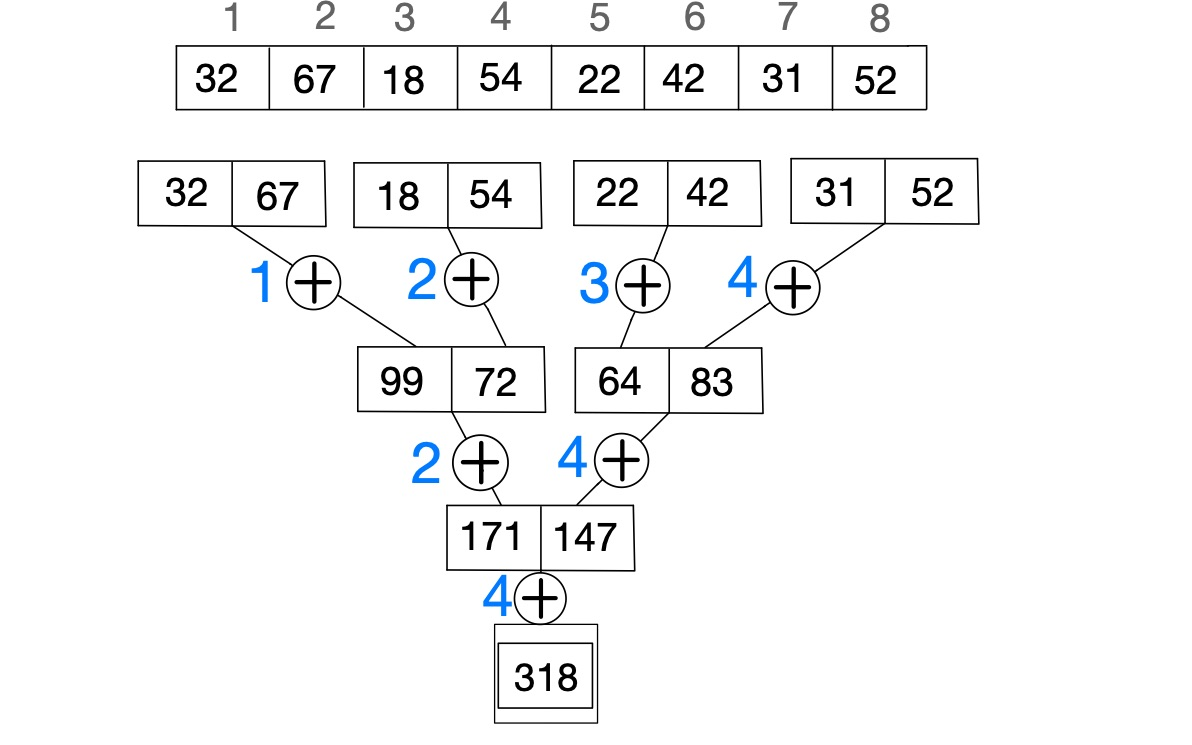
\includegraphics[width=6cm, height=7cm]{p_prefix}
	\resizebox{10cm}{!}{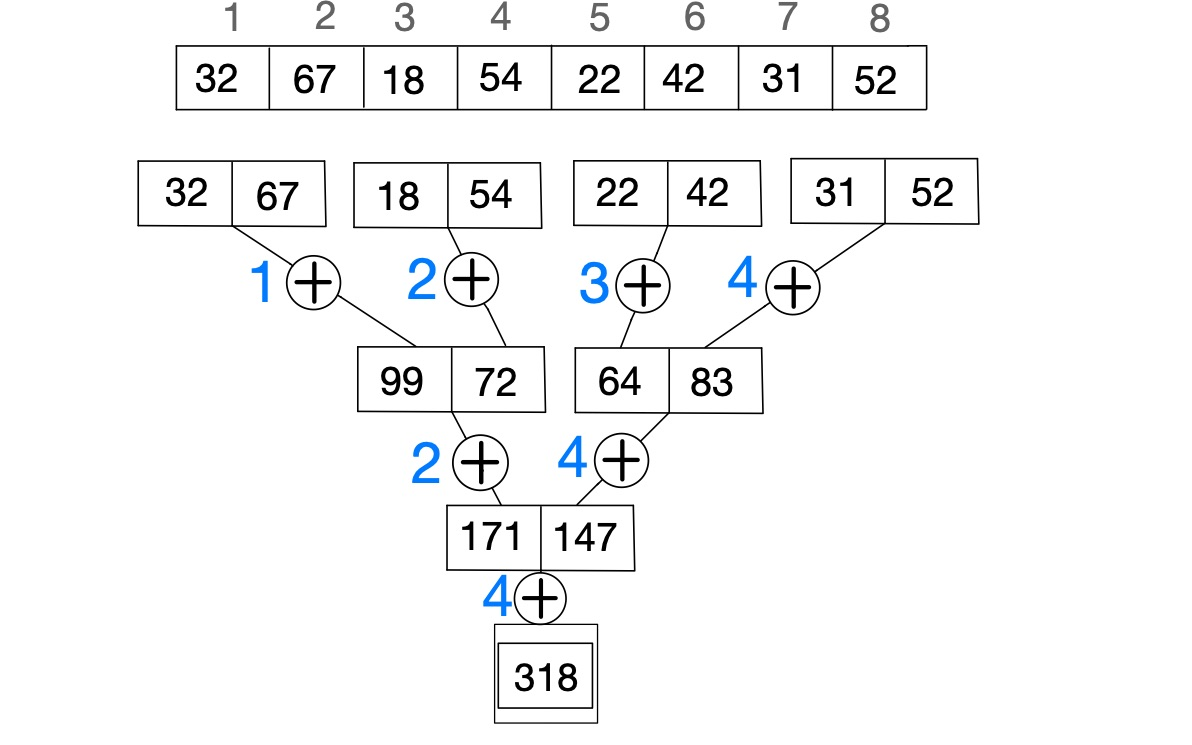
\includegraphics{p_prefix}}
	\caption{Parallel Sum}
	\label{fig:p_sum}
\end{figure}

\subsection{Parallel Practice}

Parallel programming introduces a layer of complexity that takes some time to get used to. My first experience with parallel programming was working in the C++ \textit{POSIX threads} library. 

The following is an example of a function \texttt{vecSum}. It that takes a \texttt{vector, total,} and \texttt{window} into the vector as parameters. Threads 1 and 2 are each passed the function  \texttt{vecSum} and two different windows. After  \texttt{thread2.join()} has been executed, both threads have completed their task. 

\begin{lstlisting}
#include <iostream>
#include <thread>
#include <vector>

void vecSum(std::vector<int> &v, int &total, 
        int window_begin, int window_end) {
            
  for (int i = window_begin; i < window_end; i++) {
      total += v[i];
  }
}

int main() {

  std::vector<int> vec = {1,2,3,4,5,6,7,8};
  int total_1, total_2 = 0;
  int size = vec.size();

  std::thread thread1 {vecSum, vec, total_1,0, size/2}; 
  std::thread thread2 {vecSum, vec, total_2,size/2, size};
  thread1.join();
  thread2.join();
  int total = total_1 + total_2;

  std::cout << "The vector sum is " << total << std::endl;
  return 318;
}

\end{lstlisting}

A slightly more complex example shows what happens when two or more threads need to alter the same data at the same time. When this happens without proper care, behavior is undefined and results are often far from what they were expected. To solve this, we need a lock to protect the necessary value(s) from being accessed at the same time. In C++, this comes from the \textit{mutex} library. In this example, two processors are incrementing a shared counter variable. To protect it against parallel alterations, the mutex is included when creating the custom type for storing the counter. When  \texttt{mutex.lock} is called by a processor, no other processor can access the values inside of that object until  \texttt{mutex.unlock} is called.

\begin{lstlisting}
#include <iostream>
#include <thread>
#include <mutex>

struct inc_arg_t {
  int howmany;
  int counter;
  std::mutex lock;
  inc_arg_t(int hm) : howmany {hm}, counter {0}, lock {} {}
};

void increment(inc_arg_t* arg) {
  for (int i = 0; i < arg->howmany; i++) {
    arg->lock.lock();
    arg->counter++;
    arg->lock.unlock();
  }
}

int main() {

  inc_arg_t arg { 1000000 };

  std::thread thread1 {increment, &arg};
  std::thread thread2 {increment, &arg};
  thread1.join();
  thread2.join();

  std::cout << "1000000 + 1000000 == " << arg.counter << std::endl;
  return 318;
}

\end{lstlisting}

These examples serve to illustrate the kind of coding we'll need in chapter 4 when we give a parallel implementation of graphlet census.

	\chapter{Graphlet Census With G-Tries}
	
Graphlet-tries are the tool we'll be using to implement our sequential solution. A \textit{graphlet-trie (g-trie)} is defined as a structure used to store graphlets in the shape of a tree. Recall Figure \ref{fig:motif_shapes} where we showed all possible motifs of sizes one through four. This is the visual representation of a graphlet-trie. Each node in the g-trie stores a graphlet. The top node stores the graphlet consisting of a single vertex. The node below it stores the graphlet with two vertices (an edge). This node is the parent of two nodes of size 3 and each of those is the parent of three nodes of size 4. We refer to sibling nodes as those that share a parent. The latest vertex in a sibling node has a different relationship with the vertices inherited from its parent. For example, a triangle and two star share a parent, and therefore share multiple edges and vertices. Where they differ is the latest vertex of a two star is missing the connection to the first vertex that a triangle has.

In our implementation, each node holds a certain amount of information. The most important being \texttt{IsGraphlet} and adjacency matrix \texttt{A}. \texttt{IsGraphlet} is a boolean used to determine if a graphlet is one we are interested in counting. When false, we know the current graphlet is only a middle man between us and deeper graphlets of interest. Recall the prefix trie in Figure \ref{fig:trie}; "ap" is not considered a valid english word, but "app" is. \texttt{A} is an adjacency matrix that serves to check if the newest vertex has the necessary connections to the vertices in the current search path.

\section{My Implementation}

To further orient ourselves to what is going on, let's take a bird's eye view of the algorithm before doing a deeper dive. The algorithm's search walks through the graph, along a path of vertices. As it does so, it works its way down the g-trie, going down one level each time it extends the path. At any given point, it has walked some path $p$ and is within some g-trie node $x$. If  that $x$ corresponds to a graphlet $g$ that we are interested in counting, we include $(p,g)$ in the census. From here, the idea is to be careful about how we extend $p$ with candidate matching vertices $v$. We take steps further to $v$ whenever $G / p \dot v$ corresponds to the graphlet of a child g-trie node $c$ of $x$.

Looking at the code, (line 4) of \texttt{Match} takes that next step, then seeks to repeat this \texttt{Match} step recursively with each child $c$ of $x$. This happens in the loop of (lines 7-8) of \texttt{Match}. (Line 2) of \texttt{Match} is where we find vertices $v$ that work for the subgraph of our current node $x$. There we rely on \texttt{MatchingVertices}  (which calls \texttt{CandidateCreator}) to find these valid path extensions. 

We start with an empty path and the trivial trie node. We then create a collection of vertices to match the current trie node we are in search of. Since our search is just beginning, we only need to construct a singular node,  corresponding to one graph vertex. Because of this, all graph vertices are matches. In a way, these are just the seeds of a depth-first walk through $G$ in search of our graphlets. The depth-first search is guided by the g-trie. We then check if this is a node of interest; if so, we output the current path. We continue this for the current trie node's children until we have reached the maximum node size. In our case, this occurs at size four. Once we have reached our maximum depth, we go back up one level and continue the search with the remaining matches at that level. Following the pattern of a depth first search, eventually we run through all paths starting with the initial vertex. We then move on to the next potential start vertex and continue until all possible paths have been exhausted.

Algorithm \ref{alg:seq} provides a method for finding and counting all occurrences of the g-trie nodes as induced subgraphs of an inputted graph $G$. Recall, the core benefit of a tree structure is the ability to find partial matches for potential graphlets and being able to continue searching without starting from scratch.

We start with an initial call to \texttt{GTrieMatch} with the root node of our g-trie and a graph $G$. Each child of the trie node is then passed to \texttt{Match} with an empty list representing the current partial match of vertices in a g-trie path. On (line 2) of \texttt{Match}, \texttt{MatchingVertices} is called to gather all vertices that match the current g-trie node, $x$. If $x$ corresponds to a motif of interest, then we output that graphlet occurrence (lines 4 and 5). Next we make a recursive call to \texttt{Match} on all g-trie nodes that are children
of the current node $x$. 

Let's take a deeper look into the functionality of \texttt{MatchingVertices}. On (line 2), we see a call to \texttt{CandidateCreator}. If the current path (\texttt{p}) is empty, all vertices of $G$ are candidates. An empty path means that we are just starting our graphlet search at some place in the graph. In that situation, all vertices are possible matches. This is because we are working from the root g-trie node and a match is comprised of a single vertex. In general, if the current path is not empty, then we collect all neighbors of the vertices in the current path (that are not already in the path). We then repeat this by collecting all of the non-path neighbors of the vertices in the candidate pool. Once we return back to \texttt{MatchingVertices}, we use \texttt{CheckConnections} to check each candidate's relationship to the current path (MV line 5). If a candidate vertex matches the required relationship to each of the vertices in the current path, it is added to the set of matching vertices. In the code, \texttt{CheckConnections} does this check by comparing the adjacency matrix of $x$ with the adjacency matrix of $G$. The adjacency matrix for $G$ is a $|V| \times |V|$ matrix for all possible edges in $G$. Since the adjacency matrix of a g-trie node $x$ is shared as a sub-matrix of all of the g-trie nodes that are ancestors of $x$, we only need to store a row of the adjacency matrix at each g-trie node.


For example, if $x$ were a triangle, the current path would have two vertices. Since a triangle is constructed of three vertices, with each being connected to the other two, the required adjacency matrix would be $\{1,1,0\}$. The newest vertex would need to connect to each of the prior vertices without a self-looping edge. This is implemented in the actual code, but instead denoted as $G \setminus p \sim x.graphlet$ in the pseudocode (MV line 5).

Let's take another look at (line 5) of \texttt{Match}. In the previous chapter, we pointed out that the naive solution is incorrect because it does not account for duplicates. Without symmetry-breaking conditions, there are still a few ways to protect against this. In my implementation, I stored a sorted version of the current path in a C++ \textit{set} object to avoid duplicates being counted.
	
\begin{algorithm}
\caption{Census of sub-graphs of $x$ in graph $G$}
\label{alg:seq}

\begin{algorithmic}[1]
\Procedure{GTrieMatch}{$x,G$}
    \For{children $c$ of $x$}
        \State \Call{Match}{$c,\emptyset$}
    \EndFor
\EndProcedure
\end{algorithmic}
\ \vspace{0.25in}

\begin{algorithmic}[1]
\Procedure{Match}{$x,p$}
\State $M$ := \Call{MatchingVertices}{$x,p$}
\For{$v \in M$}
    \State $p' = p \cdot v$
    \If{$x.isGraphlet$} %isgraph/isgraphlet/iscounted...etc
        \State output $p'$  \Comment{Indicates that we have found a match}
    \EndIf
    \For{children $c$ of $x$}
        \State \Call{Match}{$c,p'$}
    \EndFor
\EndFor
\EndProcedure
\end{algorithmic}
\ \vspace{0.25in}

\begin{algorithmic}[1]
\Function{MatchingVertices}{$T,p$}
\State $M = \emptyset$
\State $C := \Call{CandidateCreator}{p}$
\For{$v \in C$}
    \If{$G \setminus p \sim x.graphlet$} %going to have to explain this in the text
        \State $M := M \cup \{v\}$
    \EndIf
\EndFor
\State \Return M
\EndFunction
\end{algorithmic}
\ \vspace{0.25in}

\begin{algorithmic}[1]
\Function{CandidateCreator}{$p$}
\If{$p = \emptyset$}
    \State $C$ := $V(G)$
\Else
    \State $C := \{v : v \in N{(p)}\}$
    \State $C := C \cup \{v : v \in N{(C)}\}$
    \State \Return $C$
    
\EndIf
\EndFunction
\end{algorithmic}

\end{algorithm}

\section{Different Faces of a G-trie}
For this sequential solution, I followed the pseudocode from \citeauthor{g_tries} \cite{g_tries} pretty closely. Like any pseudocode, there was room for choices to be made in my implementation. These choices are typically made for style, efficiency, readability, and/or ease of debugging. In this section, we will discuss some of the implementation decisions I made along the way. One of the first decisions I had to make was choosing not to use \textit{canonical form}.
%%need to be consistent on whether to italicize the first mention or 2nd
Canonical form is the simplest way to represent an object in which it can be uniquely identified\footnote{Canonical form can also be used to solve the graph isomorphism problem. Two graphs are isomorphic if and only if they have the same canonical form.}. \citeauthor{g_tries} used it to reduce the size and complexity of an inputted graph. Because of this, not only does the size of the graph decrease, but it also reduces the number of duplicate calculations. \citeauthor{g_tries} \cite{g_tries}  go into more detail about specific forms they decided were optimal for this use case.

The sequential g-trie paper  by \citeauthor{g_tries} \cite{g_tries} has more details on a custom heuristic function they used to create the graphlet trie. In summary, this can be useful for use cases where specific motifs are not as important as getting a sense for the structure of a network. In other cases, such as cell-network analysis, the motifs are crucial to the search itself and must be customized. My research includes all motifs of size three and four, resulting in a trie structured like Figure \ref{fig:motif_shapes}.

Another decision I made was in \texttt{MatchingVertices}. I decided for readability, to split the core functions of \texttt{MatchingVertices} into \texttt{CandidateCreator} and \texttt{CheckConnections}. In candidate creation, \citeauthor{g_tries} \cite{g_tries} decided: from the neighbors of all $v \in p$, they selected the neighbor with the smallest neighborhood. Instead my solution collects all neighbors of every $v \in p$ not already in \texttt{p}. From there I included all of their neighbors to ensure that every possible path was considered. In chapter 5, we talk more about this being a point of optimization and continuation for this line of research.

\section{Examples} \label{sec:seq_ex}

\begin{figure}[h]
	\centering
	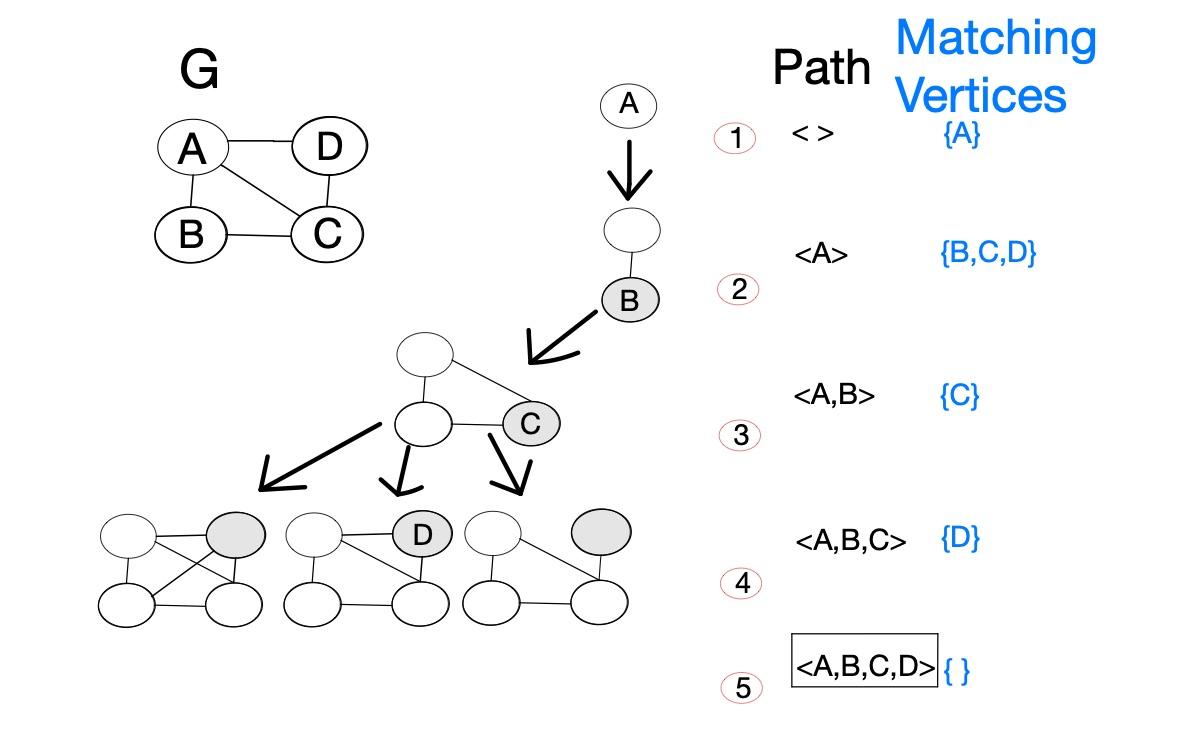
\includegraphics[width=10cm, height=8cm]{seq_walk_1}
	\caption{Sequential Walk}
	\label{fig:walk_1}
\end{figure}
For the following examples, only graphlets of size 4 are considered motifs of interest. The only thing this changes is simplifying how many times we must output a current path.

\subsection{An example walk through}
In Figure \ref{fig:walk_1}, We start with a walk through example, followed by a larger one in figures \ref{fig:walk_2}, \ref{fig:walk_3} and \ref{fig:walk_4}. Figure \ref{fig:walk_1} depicts a graph $G$, g-trie, current path, and a set of matching vertices. The circled numbers indicate the current step in the walk through. 
	
%--{try to Figure out how to do the same bolded circle number for steps and the actual graph}--
In the sequential solution, we only keep track of the matching vertices at the current depth. At each step, the g-trie node highlights the most recent addition to the current path. At step $\{1\}$, \texttt{p} is empty and $A$ is our lone vertex. At step $\{2\}$, we see that $\{A\}$ has two neighbors, $\{B, C\}$ and $B$ is chosen. Step $\{3\}$ follows similarly. At the end of step $\{4\}$, we have found an induced graphlet of size 4! Because of this, step $\{5\}$ outputs the current path of $<A,B,C,D>$.
	
\subsection{A longer walk through} \label{sec:longer_walk}
\begin{figure}[h]
	\centering
	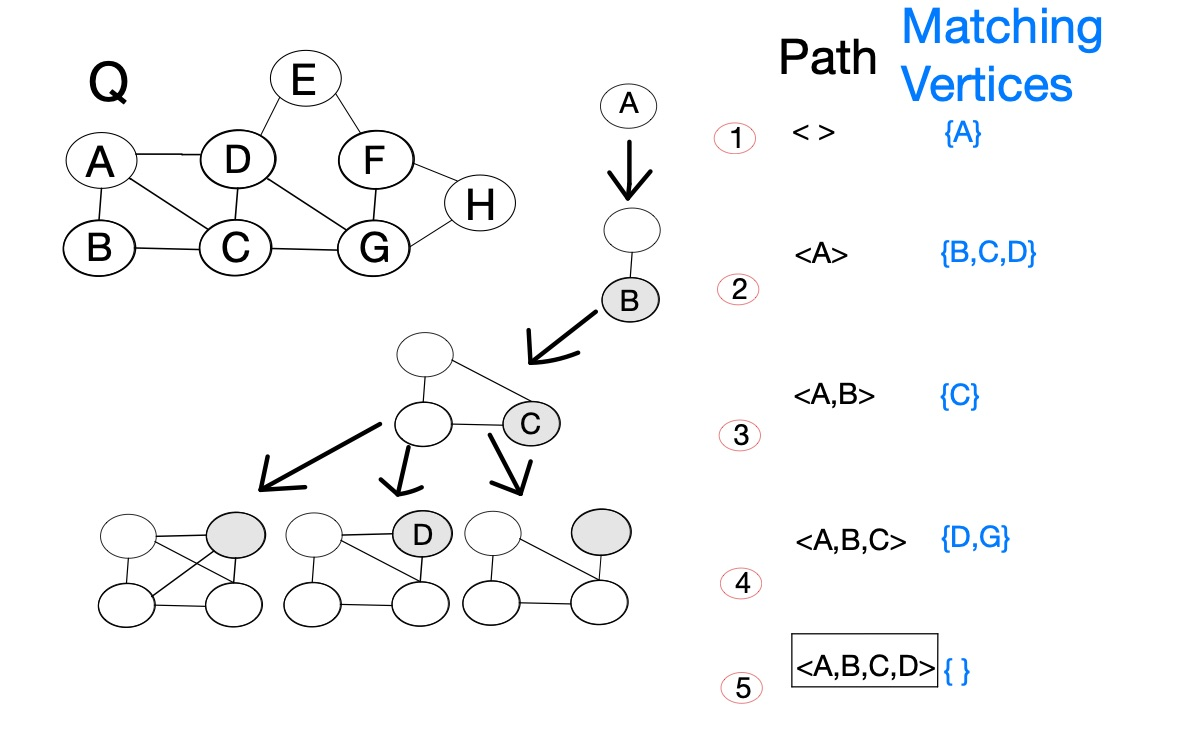
\includegraphics[width=10cm, height=8cm]{seq_walk_2}
	\caption{Larger Sequential Walk}
	\label{fig:walk_2}
\end{figure}

\begin{figure}[h!]
	\centering
	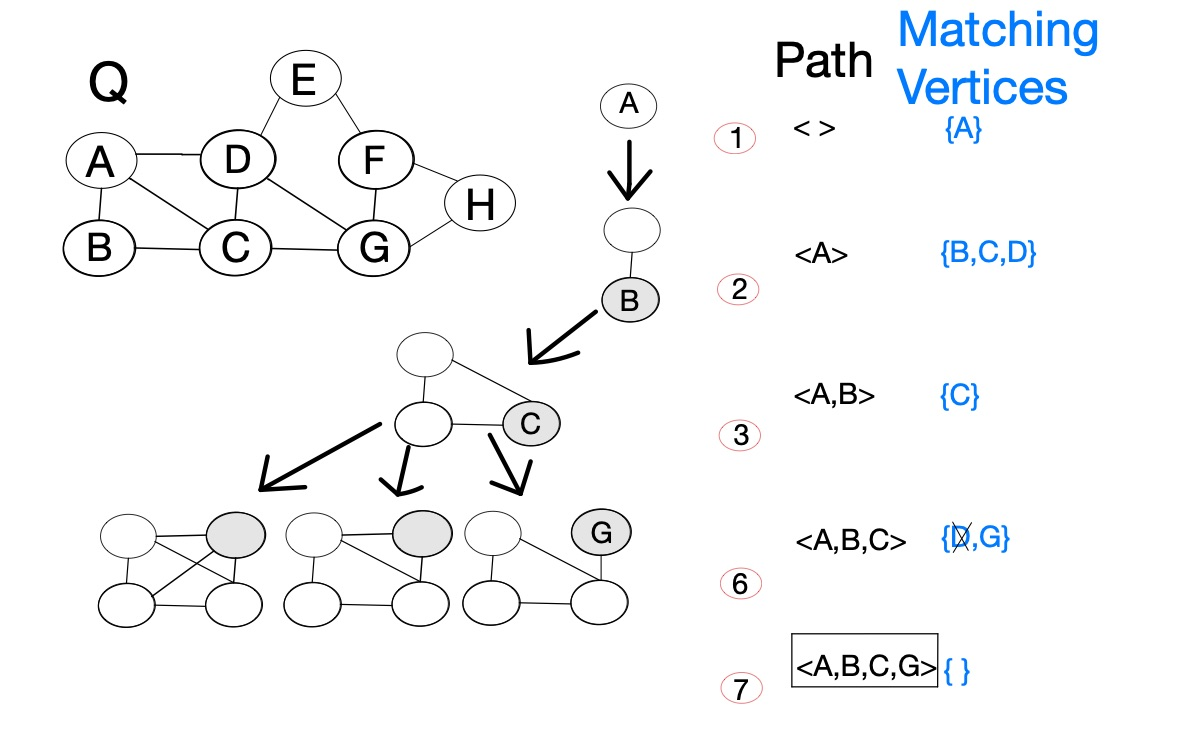
\includegraphics[width=10cm, height=8cm]{seq_walk_3}
	\caption{Larger Sequential Walk Snapshot}
	\label{fig:walk_3} %walk_3 is just showing that we crossed out the one we have already processed
\end{figure}
Figures \ref{fig:walk_2}, \ref{fig:walk_3} and \ref{fig:walk_4} show us a more complex example using graph $Q$. Steps $\{1\}$ through $\{5\}$ of Figure \ref{fig:walk_2} follow the same as Figure \ref{fig:walk_1}. At the conclusion of step $\{5\}$, we have reached the maximum depth for graphlets of interest. Now we step back up one level and see that there exists an unexplored path. Step $\{6\}$ in Figure \ref{fig:walk_3} shows the current status of us returning to level $\{4\}$ and moving past the previously explored path at the current depth. $D$ is crossed out, the previous path $<A,B,C>$ continues with $G$. This gives us a different graphlet than the one outputted in Figure \ref{fig:walk_2}.

\begin{figure}[h]
	\centering
	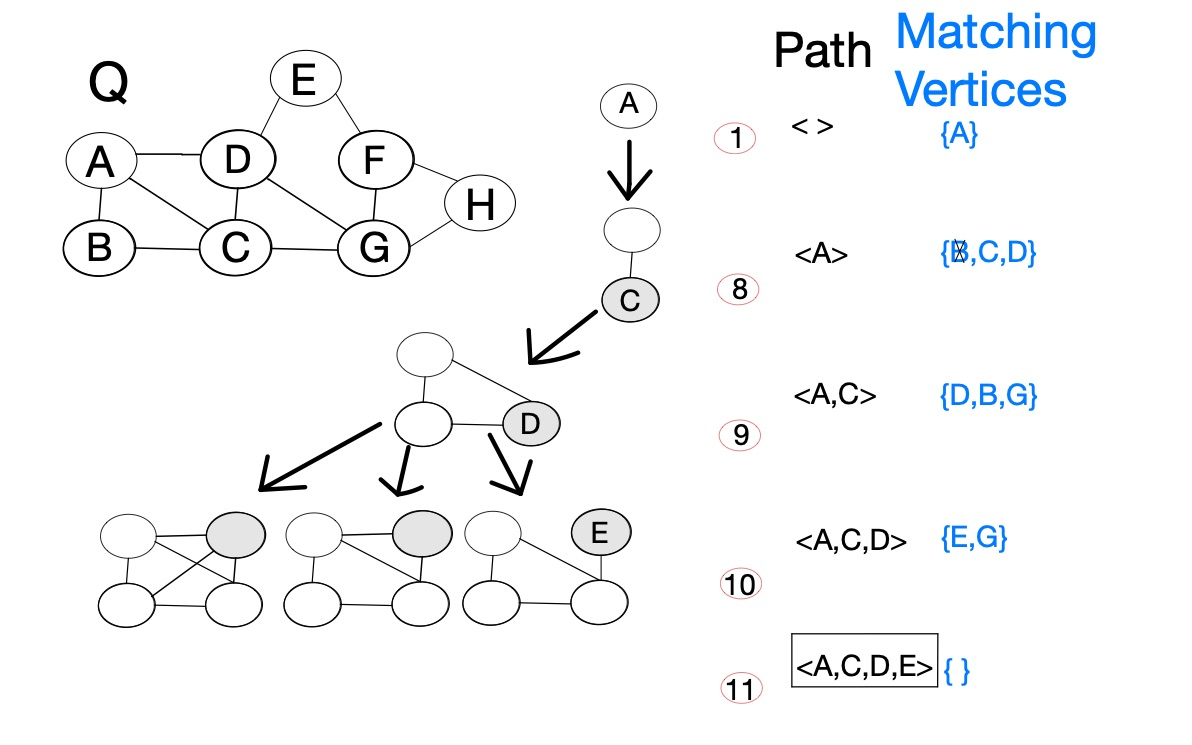
\includegraphics[width=10cm, height=8cm]{seq_walk_4}
	\caption{Larger Sequential Walk Continued}
	\label{fig:walk_4}
\end{figure}

In Figure \ref{fig:walk_4}, we continue through the rest of its neighbors that weren't selected. This gives us a new outputted graphlet of $\{A,C,D,E\}$. From there we go even further back up the stack to process through potential paths in the same fashion as Depth First Search. When all neighbors of $A$ have been fully processed, we return to (line 3) of \texttt{Match} and continue with the second vertex returned from \texttt{MatchingVertices} and so on. Recall, since the root of the g-trie is a node, the next path would start with a singular vertex.

\begin{figure}[h]
	\centering
	\resizebox{2.5cm}{!}{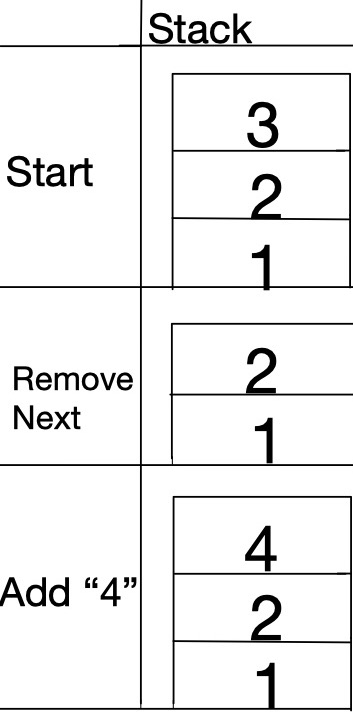
\includegraphics{stack}}
	%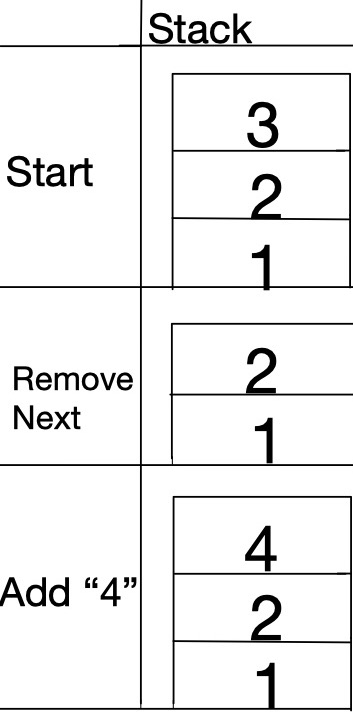
\includegraphics[width=2cm, height=3cm]{stack}
	\caption{Stack Example}
	\label{fig:stack}
\end{figure}

The concept of working back up through previous levels is known as a \textit{stack}. A stack is a collection of objects processed in a particular order. Think of a stack of pancakes. Putting them on a plate, the first pancake goes on the bottom, second on top of the first, third on top of the second and so on. Eating one at a time means that you eat the topmost (most recent) pancake, then the second, and so on. See Figure \ref{fig:stack} for an example. Objects $1,2,$ and $3$ are placed on the stack in that order. When removing from the stack, $3$ is removed first. When adding a new object $4$ to the stack, it is added to the top and will be next in line to be removed.

The importance of symmetry breaking conditions is shown again here. There are different ways to come across the same graphlet. When we return up the stack, there will be different routes to the same path (such as the triangle $\{0,1,2\}$ also being found as $\{0,2,1\}, \{2,0,1\}$, and so on). Our algorithm handles this by using C++ \textit{set} objects to maintain no duplicates being stored in the GDD counter. We will talk in chapter 5  about what an optimized setup would look like with symmetry breaking conditions.



%\section{performance}
%If I bring this back to life, I can loosely compare it to trie-less model?
%Will be moving this elsewhere

	\chapter{Parallel Census G-Tries}
	
%#refer back to sequential algorithm
%#explain general concept of algorithm without work sharing
%#explain how my process went with working on this
Following the completion of the sequential algorithm, we set our sights on a parallel solution. We worked on two models: one with work sharing and one without. \textit{Work sharing} is defined as simply as it is named: when one processor is done with its work, it asks for more from one of the processors still grinding away. The goal is to share work as seamlessly as the Christmas card example at the beginning of section \ref{sec:pre_para}.



\section{Without Work Sharing}
%#What changed from sequential
%	#change in how initial allocation is made in matching_vertices
%	#fundamental difference of how we understand the algorithm
%		#explain how each processor handles its work load

%#spread out work
%#each processor has it's own subsection of potential start vertices
\begin{algorithm}
\caption{Parallel Census}\label{alg:cap}

\begin{algorithmic}[1]
\Function{ParallelCandidateCreator}{$p, processor_{id}$}
\If{$p = \emptyset$}
    \For{$i = processor_{id}, i < |Vertices|, i += \textbf{P}$}
        \State{$C :=  C \cup  G{(V)}[i]$}
    \EndFor
\Else
    \State $C := \{v : v \in N{(p)}\footnote{The notation N(q) represents the neighbors of q not already in \texttt{p}} \}$
    \State $C := C \cup \{v : v \in N{(C)} \}$
    \State \Return $C$

\EndIf
\EndFunction
\end{algorithmic}
\end{algorithm}
Transitioning from sequential code to an initial parallel solution did not require many changes to the fundamental approach. To create a parallel algorithm, we start by looking at the functionality within \texttt{MatchingVertices}, more specifically, \texttt{CandidateCreator}. In the sequential solution, when \texttt{path} is empty, all vertices within the graph are listed as candidates. For our parallel version, this initial allocation is divided up by the number of processor round-robin style, similar to what was done by \citeauthor{par_t} \cite{par_t}. If there are 100 vertices and 10 processors, processor 1 will get vertices 1,11,21..., processor 2 will get 2,12,22... and so on. This division means that each processor will have its own set of starting vertices as it scans for motifs of interest. At the top level of the algorithm, \texttt{GTrieMatch} is called for each processor, and they each conduct an independent search with their unique search pool of starting vertices. This shows what would happen if we modified the existing structure. In the following section, we discuss a different style better suited for work sharing.

%#should we make reference to speedup scale or no? Or just save all of that for results? Is this fine as is? Maybe do performance as subsection for each
While the parallel approach offers significant improvement over the sequential algorithm, it still has room for improvement. For example, there is no easy way to evenly divide the work amongst processors. In my implementation, vertices are serialized as they are read in from a source file. While the original vertex set may be comprised of $\{31,42,75\}$, these vertices would be relabeled $\{1,2,3\}$. This is important because it means that all $P$ processors start with a search pool of $|V| / P$ vertices. Although they each start with the same number of vertices to work from, this is no guarantee of an even workload. Every graph vertex has between $0$ and $|V|-1$ neighbors. This normally leads to some processors having much more work than others, resulting in some processors finishing sooner than others. Think back to the Christmas card example at the top of section \ref{sec:pre_para}. What if, instead of a 50--50 split, the cards were divided 95--5. On top of that, you and your friend are working in separate buildings, with no means of communication or ability to share unfinished cards. These are the current working conditions faced by the processors. It makes sense to work towards a solution where a processor can ask for more work once it completes its initial allocation.
\section{Work Sharing}
%%%%%%%%%%%%%%%%%%%%
%Intro with description of what happens in work sharing, then transition into what it looks like when we transition sequential code to this style
The model we adapted for work sharing continues a similar process to what we have done thus far. However, we have structured it in a way that is more intuitive and allows for straightforward communication amongst processors. Before diving into our work sharing implementation, let's start with a new implementation of our sequential algorithm to help build an intuition for what is going on. This work relies on a \textit{work queue}. 

The work sharing graphlet paper by \citeauthor{par_t} \cite{par_t}  introduced the work queue as a means to facilitate communication between processors. Each processor is assigned a work unit. The work unit, roughly speaking, contains all the information needed to describe a snapshot of the sequential depth first search in progress. When a processor finishes its initial search, it makes a request to the global work queue, waiting until another processor is able to stop and share work. The values returned from \texttt{MatchingVertices}, current depth, path, and a set of unexplored nodes are all essential pieces of information stored in the work unit. It also stores the current g-trie node of interest. Localizing this information to each processor allows for fluid communication amongst them. Before discussing the algorithm, let's develop an understanding of how each piece of information is stored and why.

The structure \texttt{w.matches} represents the values returned from \texttt{MatchingVertices} (line 12). It is separated by depth to keep track of what would be the recursive stack. We store a numerical value as \texttt{w.depth} to represent the length of the current path. The current g-trie node of interest is stored as \texttt{w.currnode}. This retains the same level of information as it did in the sequential algorithm (such as \texttt{isGraphlet}). Lastly, \texttt{w.gnodes} stores the next round of nodes to explore. Similar to \texttt{w.matches}, this is also stored by depth. At depth $n$, our path has size $n$. Our current node is the corresponding g-trie node to our path. At this depth, our \texttt{gnodes} are children of the current node. For example, suppose we are at depth three with the current node being a triangle. \texttt{w.gnodes} would consist of its three child nodes.
%save this for algorithm walk through
%Sticking with our example of a triangle, suppose the current triangle has a path of $1,2,3$.
\subsection{Alternative Sequential Implementation}

Algorithm \ref{alg:alt_seq} shows this sequential adaptation. Instead of recursive calls to \texttt{Match}, we've implemented a looping search dependent on our current depth. If depth equals zero, then we know the search has been completed. \texttt{Count} is passed a work unit \texttt{w}. The current node begins with the root trie node, which is equivalent to the empty string in a prefix trie. Since the node at depth $1$ consists of a singular graph vertex, \texttt{w.matches} is populated with all $v \in V(G)$. 

(Line 4) pulls the first matching vertex at the current depth. We then increment depth (line 6)  and check if the current node is one of interest (lines 7-8). We then populate \texttt{gnodes} at our new depth with the children of our current node (line 9). This process repeats until we get to the maximum depth allowed by the current path. Once we reach that depth, \texttt{matches} and \texttt{gnodes} are both empty, therefore we remove the latest node from the end of our current path (line 14) and decrement depth (line 15). This returns us up one level in the call stack.

A snapshot into the algorithm would look as follows: suppose the maximum path depth for our first search ended on a \textit{4-clique}. Removing the last vertex moves us back up to a triangle. The current node is triangle. Each matching vertex in \texttt{matches} forms a 4-clique with the current path, and \texttt{gnodes} is populated with the remaining children of a triangle. We repeat the condition from (lines 3-9) until all potential cliques with the current path are found. Once the matches at depth $3$ have been exhausted, we jump down to (lines 10-12) where we pull in the next child node of a triangle, populate \texttt{matches} accordingly, and repeat (lines 3-9) for this new node. Once we have exhausted the children of a triangle, we step back up to its parent node (edge) and repeat.

Similar to Algorithm \ref{alg:seq}, we can use this same structure to implement a parallel search without work sharing. The initial allocation of vertices is the only substantial change. Each processor makes a different call to \texttt{Count}, performing an independent search with a unique set of initial matches.



\begin{algorithm}
\caption{Alternate Graphlet Census}\label{alg:alt_seq}
\begin{algorithmic}[1]
\Procedure{Count}{$w$}
    \While{$w.depth > 0$ }
        \If{$w.matches[w.depth] \neq \emptyset$}
            \State$v := \Call{nextMatch}{w.matches[w.depth]} $
            \State $\Call{pushPath}{w.path,v}$
            \State $w.depth = w.depth + 1$
            \If{$w.currnode.isGraphlet$}
                \State $\Call{output}{w.currnode, w.path}$
            \EndIf
            \State $w.gnodes[w.depth] :=  \Call{children}{w.currnode}$
        \ElsIf{$w.gnodes[w.depth] \neq \emptyset$}
            \State $w.currnode = \Call{nextGnode}{w.gnodes[w.depth]}$
            \State $w.matches[w.depth] =   \Call{MatchingVertices}{w.path,w.gnodes} $
        \Else
            \State $\Call{popPath}{w.path}$
            \State $w.depth = w.depth - 1$
        \EndIf
    \EndWhile
\EndProcedure
\end{algorithmic}
\end{algorithm}

\subsection{Work Sharing Implementation}
%talk about how the previous work set us up for easy work sharing then go into implementation
%Can also have subsection talking about specifics of my implementation such as sorting before storing

%introduce work sharing functions here then show how they play into bigger picture
Before seeing how the alternative sequential algorithm is modified into one with intuitive work sharing, we must define the functions that make work sharing possible. \texttt{AskForWork} and \texttt{OfferWork}. When a processor has completed its initial workload, it makes a request for more work. This sends a message to the other processors, requesting one of them to share their remaining workload with the requester. \texttt{OfferWork} begins by checking if there are any active requests for work. If so, then it pulls in a request and splits its \texttt{matches} at each level in half to share with the requesting processor. The new processor receives a copy of the sender's \texttt{gnodes}, current node, and path. This is because they both resume working from where the sender is currently at. The split in matching vertices allows them to explore different paths branching from the same start path. We see an example of this in section \ref{sec:comp_ex}. 

We see the work sharing approach implemented in Algorithm \ref{alg:ws}. The only change at this level is the addition of a new conditional check based on the current depth (lines 16-20). When depth equals zero, then the  processor has completed its current workload. It then makes a request for more work and updates its depth to match its new path. If a processor has not completed its work, it checks to see if there are any pending requests currently. 

\begin{algorithm}
\caption{Work Sharing Graphlet Census}\label{alg:ws}
\begin{algorithmic}[1]
\Procedure{ParallelCount}{$w$}
    \While{$w.depth > 0$ }
        \If{$w.matches[w.depth] \neq \emptyset$}
            \State$v := \Call{nextMatch}{w.matches[w.depth]} $
            \State $\Call{pushPath}{w.path,v}$
            \State $w.depth = w.depth + 1$
            \If{$w.currnode.isGraphlet$}
                \State $\Call{output}{w.currnode, w.path}$
            \EndIf
            \State $w.gnodes[w.depth] :=  \Call{children}{w.currnode}$
        \ElsIf{$w.gnodes[w.depth] \neq \emptyset$}
            \State $w.currnode = \Call{nextGnode}{w.gnodes[w.depth]}$
            \State $w.matches[w.depth] =   \Call{MatchingVertices}{w.path,w.gnodes} $
        \Else
            \State $\Call{popPath}{w.path}$
            \State $w.depth = w.depth - 1$
        \EndIf
        \If{$w.depth = 0$}
            \State $\Call{AskForWork}{w}$
            \State $w.depth = |w.path|$
        \Else
            \State $\Call{OfferWork}{w}$
        \EndIf
    \EndWhile
\EndProcedure
\end{algorithmic}
\end{algorithm}

%%%%%%%%%%%%%%%%%%%%




%defining helper functions
%explaining their useful-ness
%setting up another walk through (after cleaning this up, I can draw it on the iPad)
%can include a small re-showing of the sequential algorithm for showing the changes made (can include references for without w/s too)

\subsection{Beyond the Pseudocode}
To properly share my experience, it is helpful to provide some additional context. My experience working from the work sharing pseudocode from \citeauthor{par_t} \cite{par_t} left even more room for implementation choice when compared to the sequential algorithm. For example, \citeauthor{par_t} \cite{par_t} constructed a work unit using one continuous array to store current depth, \texttt{unexploredVertices}, \texttt{unexploredNodes} and \texttt{path}. This requires careful indexing to pass  this work array to functions \texttt{DivideWork} and \texttt{ResumeWork}. In my implementation, I used a C++ class to create a work unit object. This way, I could track the same values by name and store them with different data structure that made sense on a case-by-case basis. The change in structure shown in Algorithm \ref{alg:ws} is another example of a stylistic choice I made along the way. While it functions similarly to to the adaptation they used, my implementation simplified how the processors share and continue work after a request. This results in more readable code that is easier to debug.


\subsection{Thread-Safety}
Another important aspect of the work-sharing model is proper thread safety. The original parallel algorithm had to safeguard against multiple writes to a global GDD. This means that two processors attempted to put new paths into the GDD at the same time. Competing writes lead to undefined (and very problematic) behavior without proper protection. Initially, we fixed this by creating a thread-safe GDD object, locking access whenever one processor was actively writing to it. With frequent writes from all processors, this locking, unlocking, and associated overhead, caused large slow downs. We solved this problem by diverging from the sequential code and giving each processor a local GDD to write to. Once all calculations have been performed, these are all aggregated into one global GDD. This offered great speedups that put us a lot more in-line with the hope of linear speedups as the number of processors increases.

Once we got to the work-sharing model, thread safety became even more important. In addition to GDD, we need to now protect the mechanism in charge of handling work requests. My implementation used a \textit{global queue}. This queue object stores pointers to the work units of requesting processors. Anytime a processor checks for requests to fulfill, the requesting work unit gets dequed from the queue. We must protect against multiple processors attempting to fulfill the same request. We must also protect against parallel writes to avoid undefined behavior. Similar to our first approach for GDD, I created a custom class with a mutex to protect calls to \textit{enqueue} and {dequeue}. This protects against parallel reads and writes to the global queue.

\section{A More Complex Example} \label{sec:comp_ex}
%P = 2
% 

\begin{figure}[h]
	\caption{Parallel Walk Graph}
	\centering
	\resizebox{12cm}{!}{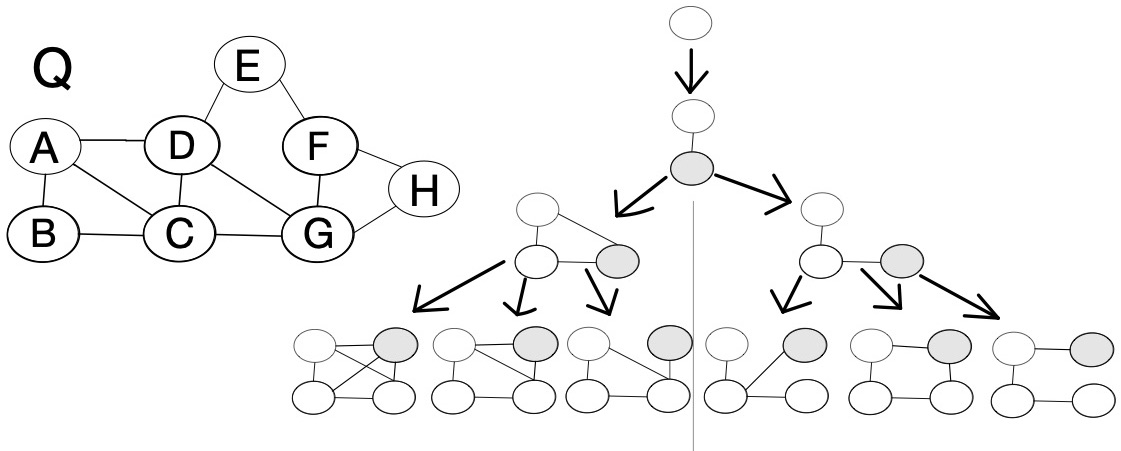
\includegraphics{par_walk_1}}
	%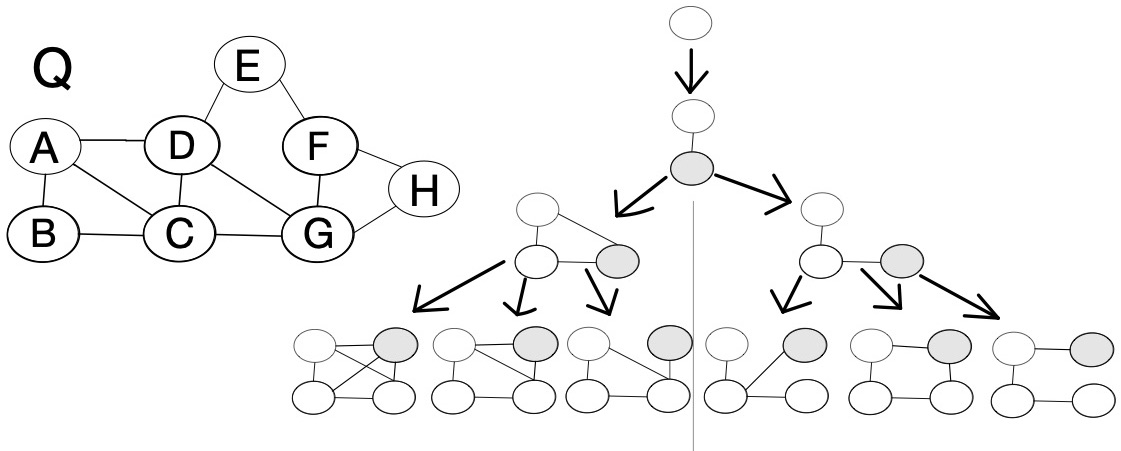
\includegraphics[width=8cm, height=6cm]{par_walk_1}
	\label{fig:par_walk_graph}
\end{figure}

Here, we show a step-by-step example of how work sharing operates. We reuse the same graph from Figure \ref{fig:walk_2}, depicted in Figure \ref{fig:par_walk_graph}. The g-trie structure is also included for convenience.


\begin{table}[h!]
%\begin{tabular}{ |p{3cm}||p{3cm}|p{3cm}||p{3cm}||p{3cm}|p{3cm}||p{3cm}| }
\begin{tabular}{ |c c c| c | c c c |  }
	 \hline
 	\multicolumn{3}{|c|}{Processor 0} &  & Processor 1\\
	%\multirow{3}{4em}{Multiple row} & cell2 & cell3
 	\hline
	 Path$_{0}$ & MatchingV$_{0}$ & Motif$_{0}$ &\textbf{Step} & Path$_{1}$ & MatchingV$_{1}$ & Motif$_{1}$ \\
 	\hline
	$<  >$ & $\{A,C,E, G\}$ & \textbf{none} &\textbf{0}& $<  >$ & $\{B, D, F, H\}$ & \textbf{none} \\
	$<A>$ & $\{C,B,D\}$ & Node &\textbf{1}& $<B>$ & $\{C,A \}$ & Node \\
	$<A,C>$ & $\{D,B\}$ & Edge &\textbf{2}& $<B,C>$ & $\{D,A,G\}$ & Edge \\
	$<A,C,D>$ & $\{E\}$ & Triangle &\textbf{3}& $<B,C,D>$ & $\{E\}$ & Two Star \\
	$<A,C,D,E>$ & $\{\}$ & Tailed Triangle &\textbf{4}& $<B,C,D,E>$ & $\{\}$ & Four Path \\
	 \hline
\end{tabular}
 \caption{Simple Census Table}
\label{table:par_1}
\end{table}

Table \ref{table:par_1} provides a walk through for the graph $Q = (\{A,B,C,D,E,F,G \}, \\ \{ (A,B), (A,C), (A,D), (B,C), (C,D), (C,G), (D,E), (D,G), (E,F), (F,G), (F,H), (G,H)\})$, when $P = 2$. At each step, processors $p_{0}$ and $p_{1}$ are given an allocation of vertices ($MatchingV$), path, and motif. Since there are two processors, $p_0$ receives the odd indexed vertices and processor 1 receives the even. The motif at step $k$ matches the path at step $k$. For example, triangle is the motif for $p_{0}$ at step 3, and the corresponding path is $\{A,C,D\}$. It also holds true that the motif at step $k$ is the shape obtained by adding the next vertex in the allocation to the path at step $k-1$. This means the $k-1$ allocation of vertices, all correspond to the motif at step $k$. At step 3, $D$ has 2 neighbors not currently in the path, $B$ and $E$. $E$ is the only allocated vertex because it is the only one that can create a Tailed Triangle at step 4.

\begin{table}[h!]
\begin{tabular}{ |c| c c c |  }
	 \hline
 	\multicolumn{4}{|c|}{Processor 0} \\
	%\multirow{3}{4em}{Multiple row} & cell2 & cell3
 	\hline
	 \textbf{Step} & Path$_{0}$ & MatchingV$_{0}$ & Motif$_{0}$ \\
 	\hline
	\textbf{0} & $<  >$ & $\{$\sout{A}$,C,E, G\}$ & \textbf{none} \\
	\textbf{1} & $<A>$ & $\{$\sout{C}$,B,D\}$ & Node \\
	\textbf{2} & $<A,C>$ & $\{$\sout{D}$,B\}$ & Edge \\
	\textbf{3} & $<A,C,D>$ & $\{$\sout{E}$\}$ & Triangle \\
	\textbf{4}& $<A,C,D,E>$ & $\{\}$ & Tailed Triangle \\
	 \hline
	 \hline
 	\multicolumn{4}{|c|}{Processor 1}\\
	%\multirow{3}{4em}{Multiple row} & cell2 & cell3
 	\hline
	 \textbf{Step} & Path$_{1}$ & MatchingV$_{1}$ & Motif$_{1}$ \\
 	\hline
	\textbf{0}& $<  >$ & $\{$\sout{B}$, D, F, H\}$ & \textbf{none} \\
	\textbf{1}& $<B>$ & $\{$\sout{C}$,A \}$ & Node \\
	\textbf{2}& $<B,C>$ & $\{$\sout{D}$,A,G\}$ & Edge \\
	\textbf{3} & $<B,C,D>$ & $\{$\sout{E}$\}$ & Two Star \\
	\textbf{4} & $<B,C,D,E>$ & $\{\}$ & Four Path \\
	 \hline
\end{tabular}
 \caption{Snapshot  after one round}
\label{table:par_cur}
\end{table}

Steps 1-4 continue similar to the sequential solution. This results in $<A,C,D,E>$ and $<B,C,D,E>$ being stored at their respective motifs. Table \ref{table:par_cur} is the current status for each processor at the conclusion of step 4. Similar to the sequential algorithm, the subsequent steps continue working up the stack until processing through the initial allocation of start vertices. We now fast forward to when things start to get interesting. At step 5 (Table \ref{table:par_ws}), $p_{0}$ has completed its work (\texttt{path} and $MatchingV$ are both empty). At step 6, $p_0$ makes a request for more work. $P_1$ then stops its work, stores its current state, and prepares to make a call to \texttt{DivideWork}.

\begin{table}[h!]
\begin{tabular}{ |c c c| c | c c c |}
	 \hline
 	\multicolumn{3}{|c|}{Processor 0} &  & Processor 1\\
	%\multirow{3}{4em}{Multiple row} & cell2 & cell3
 	\hline
	 Path$_{0}$ & MatchingV$_{0}$ & Motif$_{0}$ & \textbf{Step} & Path$_{1}$ & MatchingV$_{1}$ & Motif$_{1}$ \\
 	\hline
	$<  >$ & $\{$\sout{A,C,E, G}$\}$ & \textbf{none} &\textbf{5}& $<  >$ & $\{$\sout{B, D}$, F, H\}$ & \textbf{none} \\
	please & send & work &\textbf{6}& $<F>$ & $\{E,H,G\}$ & Node \\
	%$<  >$ & $\{\}$ & \textbf{none} &\textbf{5}& $<F>$ & $\{E, G,H\}$ & \textbf{Node} \\	 If we don't like the line above, then we can revert to this
	 \hline
\end{tabular}
 \caption{Snapshot of work being requested}
\label{table:par_ws}
\end{table}

Table \ref{table:par_shared}  shows the aftermath of this transaction. At step 8, $p_0$ has copied the current path and motif from $p_1$. They split the allocated vertices at steps 7 and 8. From here, they both resume search as normal.

\begin{table}[h!]
\begin{tabular}{ |c| c c c |  }
	 \hline
 	\multicolumn{4}{|c|}{Processor 0}  \\
	%\multirow{3}{4em}{Multiple row} & cell2 & cell3
 	\hline
	 \textbf{Step} & Path$_{0}$ & MatchingV$_{0}$ & Motif$_{0}$\\
	 \hline
	 \textbf{7}&$<  >$ & $\{H\}$ & \textbf{none} \\
	 \textbf{8}&$<F>$ & $\{G\}$ & Node \\
	 \textbf{9}&$<F,G>$ & $\{C,D\}$ & Edge \\
	 \textbf{10}&$<F,G,C>$ & $\{D\}$ & Two Star \\
	 \textbf{11}&$<F,H,G,D>$ & $\{\}$ & Tailed Triangle \\
 	\hline
	\hline
	\multicolumn{4}{|c|}{Processor 1} \\
	\hline
	\textbf{Step} & Path$_{1}$ & MatchingV$_{1}$ & Motif$_{1}$\\
	\hline
	 \textbf{7}& $<  >$ & $\{F\}$ & \textbf{none} \\
	 \textbf{8}& $<F>$ & $\{E,H\}$ & Node \\
	\textbf{9} & $<F,E>$ & $\{D\}$ & Edge \\
	 \textbf{10} & $<F,E,D>$ & $\{G,C,A\}$ & Two Star \\
	 \textbf{11} & $<F,E,D,G>$ & $\{\}$ & Square\\
	 \hline
\end{tabular}
 \caption{Snapshot after work is shared}
\label{table:par_shared}
\end{table}

\section{Performance}
While chapter 5 is dedicated to more formal performance analysis, I can use this time to tell you what my experience was. Initially, I did not see great speedups transitioning from my initial parallel code to proper work sharing. Part of this was dealing with standard debugging. But the core issue I faced was handling the shared $GDD$ between processors. Work sharing in itself does not leave much room for undefined behavior because those calls occur less frequently. Very rarely do several occur at the same time. Each processor is handling hundreds or \textit{thousands} of matches that must all be counted. This creates a lot of opportunities for parallel writes that cause undefined behavior. This causes invalid results and program crashes. Once I transitioned to a localized $GDD$ solution, my results got faster and more consistent. The additional work of aggregating the data in the end added a negligible amount of time to the total runtime. Even when using 128 threads working with a large collaboration network of astrophysicists from the Stanford Network Analysis Platform \cite{snap}, this took under 30 seconds. For context, the search itself took 40 hours with work sharing. All of this goes to say, localizing $GDD$ to each processor was the better design.



	\chapter{Results and Discussion}
	
	
	
\section{Results}

In this chapter, I describe the performance and results of running my code on sample data. I conducted final performance testing using another SNAP network. I chose the \textit{Gnutella peer-to-peer file sharing network}, collected on August 9th, 2002 \cite{snap}. I decided on this particular data set because of its vertex (8,114) to edge (26,013) ratio. I wanted a data set that would take approximately 90 minutes for the sequential solution to complete. This would allow me to do several runs, including runs with a variable number of processing threads. The sequential algorithm completed its census in 1 hour, 30 minutes, and 36 seconds. This time served as the benchmark for comparing our parallel implementations. Linear scaling is often used as a goal for parallelizing a sequential algorithm. With linear scaling, each doubling of processors results in a halving of runtime. An added benefit of choosing a SNAP data set is that it comes with triangle counts pre-calculated. This serves as an additional verification that our code is computing correct graphlet counts. All tests were run on a \textit{AMD Ryzen Threadripper 3970X} with 32 cores and two threads per core. Both parallel solutions were run three times then averaged, and their averages are compared in Figure \ref{fig:perform}.

\subsection{Analysis}

Tables \ref{table:p_perf} and 5.1.2 show performance numbers for the parallel and work sharing solutions respectively. Starting with the parallel solution, we get near linear speedups until we reach 32 threads. There isn't really a case of diminishing returns, but rather a drop off from 16 to 32 and another dip from 32 to 64. Load balancing plays a large part in the performance of this algorithm. As we discussed previously, an even distribution of initial vertices does not correspond to an even amount of work. This means that, without a method for work sharing, some threads will inevitably have much more work than others. Some threads will inevitably finish faster, while the rest are still busy at work. Workloads are more even when all graph vertices have a similar number of neighbors.
\begin{table}[h!]
\begin{tabular}{ |c | c | c | c | c | }
	 \hline
 	\multicolumn{5}{|c|}{Parallel Performance  (H:MM:SS)}\\
	%\multirow{3}{4em}{Multiple row} & cell2 & cell3
 	\hline
	 Threads & Trial 1 & Trial 2 & Trial 3 & \textbf{Average} \\
 	\hline
	1 & 1:30:54 & 1:30:56 & 1:30:50 & 1:30:54  \\
	2 & 0:48:23 & 0:48:19 & 0:48:21 & 0:48:21  \\
	4 & 0:27:41 & 0:27:49 & 0:27:39 & 0:27:43  \\
	8 & 0:14:37 & 0:14:37 & 0:14:37 & 0:14:37  \\
	16 & 0:11:28 & 0:11:28 & 0:11:28 & 0:11:28  \\
	32 & 0:07:04 & 0:07:07 & 0:07:07 & 0:07:06  \\
	64 & 0:06:47 & 0:06:47 & 0:06:47 & 0:06:47  \\
	128 & 0:04:59 & 0:05:01 & 0:05:02 & 0:05:01 \\
	 \hline
\end{tabular}
\label{table:p_perf}
\end{table}
	
For work sharing, we get near linear speedups until we go from 16 to 32 threads (as seen in Figure \ref{fig:speedups}). The overhead for my implementation of work sharing increases significantly at this point. Using print statements to see exactly when work was being exchanged, it became clear that the "first come, first served" implementation does not do well when there are frequent requests for work. For example, a thread that very recently asked for work, would be the first to offer work to another requesting thread. This leads to smaller workloads being shared, and more requests needing to be filled. For 64 and 128 threads, this certainly worked to its detriment. Another challenge faced by the run with 128 threads is hardware limitations. With only 64 hardware threads, attempting to run more than that requires tricks that are beyond the scope of this thesis. It is sufficient to say that attempting to use more threads than the hardware has available results in diminished performance.
%(maybe optimizations can include work stealing charlie mentioned)	 lmaoooo fuck outta here
\begin{table}[h!]
\begin{tabular}{ |c | c | c | c | c | }
	 \hline
 	\multicolumn{5}{|c|}{Work Sharing Performance}\\
 	\hline
	 Threads & Trial 1 & Trial 2 & Trial 3 & \textbf{Average}  \\
 	\hline
	1 & 1:24:35 & 01:25:13 & 01:24:32 & 1:24:47 \\
	\hline
	2 & 0:42:12 & 0:48:06 & 0:43:18 & 0:44:32  \\
	\hline
	4 & 0:25:54 & 0:22:00 & 0:24:12 & 0:24:02  \\
	\hline
	8 & 0:14:18 & 0:10:48 & 0:12:30 & 0:12:32  \\
	\hline
	16 & 0:06:36 & 0:06:00 & 0:06:48 & 0:06:28 \\
	\hline
	32 & 0:06:00 & 0:06:06 & 0:06:12 & 0:06:06  \\
	\hline
	64 & 0:07:12 & 0:07:06 & 0:07:18 & 0:07:12  \\
	\hline
	128 & 0:10:36 & 0:10:30 & 0:10:33 & 0:10:33 \\
	 \hline
\end{tabular}
\label{table:ws_perf}
\end{table}

\begin{figure}[h]
	\centering
	\resizebox{14cm}{!}{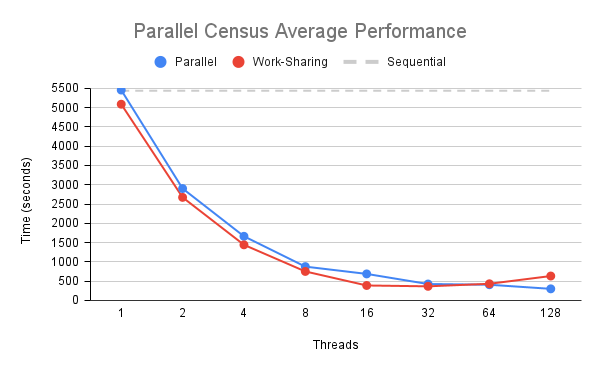
\includegraphics{performance}}
	\caption{Performance Comparison}
	\label{fig:perform}
\end{figure}

\begin{figure}[h]
	\centering
	\resizebox{14cm}{!}{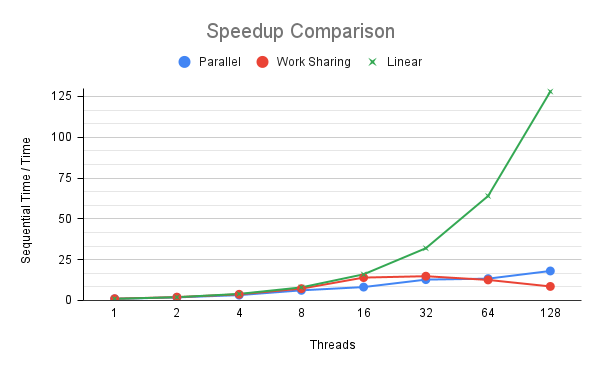
\includegraphics{speed}}
	\caption{Speedup Comparison}
	\label{fig:speed}
\end{figure}

Figure \ref{fig:perform} provides a visual of the average performance for each algorithm. The work sharing implementation consistently performs better until we get to 64 threads. At this point, they are near equal, and the original parallel solution actually performs better with 128 threads. This is evidence of the added overhead to more frequent calls to share work. Comparing the tables, it's also clear that the work sharing implementation has less consistent results. Work requests are offered and fulfilled in a different order each time the code is run. Sometimes larger work loads are among the first to be split up, which leads to a better use of processing power. Other times, work is spread by those who have less work to offer, which causes a chain of more requests. Without work sharing, each thread has the same amount of work each time it runs because there is no change to the initial allocation of vertices. This leads to more consistent results. 

Figure \ref{fig:speed} shows how close each implementation is to the goal of linear speedups. Up to 8 threads, both implementations show near-linear speedups. This continues to 16 processors for the work sharing implementation. Once we go beyond 16 threads, both fall behind.

	\section{Furthering This Research}
	%Symmetry breaking conditions
	%canonical form
	%* Minimum size req for a processor before it shares work
	%changing the time checker for messages
	%Having better distribution of neighbors
	
Through the course of this thesis, we have briefly discussed things that could be done to improve our algorithm. Now is the time for us to flesh out these ideas in more detail.

\begin{figure}[h]
	\centering
	\resizebox{8cm}{!}{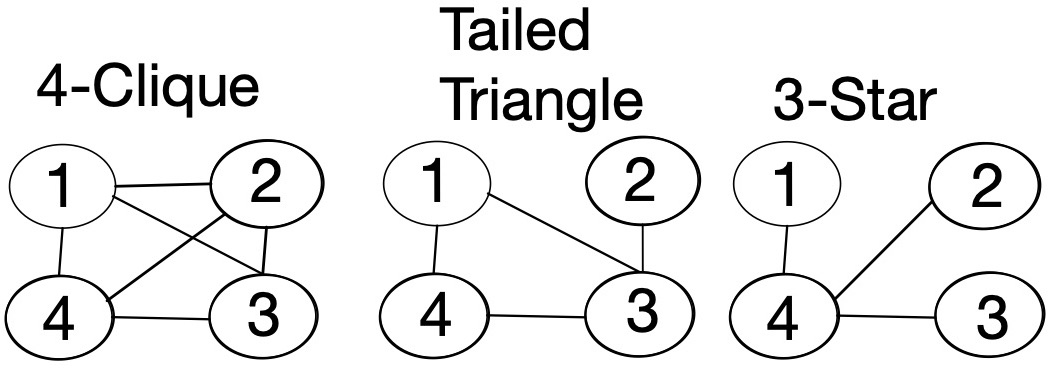
\includegraphics{motif_four}}
	\caption{Motifs of size 4 with automorphisms}
	\label{fig:aut}
\end{figure}

The first improvement mentioned is the addition of symmetry breaking conditions. For shapes with \textit{automorphisms}---an isomorphic mapping onto itself---it helps to have something in place to prevent multiple discoveries. For example, take a look at Figure \ref{fig:aut}. Here we show motifs of size four with labeled vertices. When looking at a tailed triangle, we see that vertices $1$ and $4$ could be swapped and the same shape would still hold true. Similarly, in a four clique, there exist $4!$ ways to find the same clique. \citeauthor{g_tries} \cite{g_tries} implemented a solution in which, each point of swapping is given a comparison to eliminate multiple discoveries of the same path. They decided on sorting by vertex index. For example, the tailed triangle would have the condition $(2 < 3)$. This means that any search for a tailed triangle where $(2 > 3)$ is terminated early. In the case of the four clique, its conditions would be $\{(0<1), (0<2), (0<3), (1<2),(1<3), (2<3)\}$. Each node object with automorphisms would hold its own set of symmetry breaking conditions. Conditions would be used to prevent the output of duplicate graphlets. They are also used to terminate further calls to \texttt{MatchingVertices}. On (line 3) of Algorithm \ref{alg:sc}, we see this in action. If the current path does not respect symmetry conditions, then it is no longer expanded, saving valuable time and computational resources.

\begin{algorithm}
\caption{Symmetry Conditions} \label{alg:sc}
 \begin{algorithmic}[1]
\Function{MatchingVerticesConditions}{$x,p$}
\State $M = \emptyset$
 \If{$p$ does not respect $x.conditions$} \Comment{new}
 \State \Return $\emptyset	$			\Comment{new}
\EndIf
\State $C := \Call{CandidateCreator}{p}$
\For{$v \in C$}
    \If{$G \setminus p \sim x.graphlet$} %going to have to explain this in the text
        \State $M := M \cup \{v\}$
    \EndIf
\EndFor
\State \Return M
\EndFunction
\end{algorithmic}
\end{algorithm}
 
 Another area of improvement is the optimization of our work sharing implementation. A reason for the diminishing returns in our results is the frequent calls to share work. Currently, the first processor to see a pending work request is the first one to respond to it. This lead to a lot of splitting of work when there isn't much work to be split. The increased overhead of frequent search stops could be reduced by implementing a mechanism to determine if the current work unit contains enough work that it is worth the effort of sharing. If not, then it does not attempt to offer work.
 
The work sharing solution proposed by \citeauthor{par_t} \cite{par_t}, also implemented a time check that would reduce the number of checks for incoming work by a processor. When the program first starts, every processor is busy. As some processors begin to finish their initial workload, work requests grow in number and frequency. Ideally, this time check would be a function of the graph size and number of processors. It should also be able to dynamically adjust based on the frequency of work requests at a given time. A way to measure this is to increase the time whenever there is a check for work requests that returns false. A false return means that work was offered, but no one needed work in that moment. Similarly, we would decrease the timer when more requests come back true. Reducing the total number of checks helps decrease the overhead of sharing.

\section{Conclusion}

In conclusion, the speedups provided by parallelizing the initial algorithm are a testament to the power of parallel processing. Taking a problem that took over an hour to complete, and getting it to finish in under seven minutes is no small task. Even working on a personal computer (with less than 32 cores), parallelization allowed the runtime to decrease from ninety minutes to less than fifteen. In real world applications, this would allow for much faster turnaround times, allowing for increased productivity. Compared to individually searching for shapes of interest, g-tries proved to be a much faster solution. The combination of parallelization and graphlet census showed an ability to speed up a computation that has a wide variety of meaningful applications. Whether it be social networks, biological networks, or any application involving subgraph counting, parallel graphlet census has proven to be a valuable tool.

	

%If you feel it necessary to include an appendix, it goes here.
    %\appendix
      %\chapter{The First Appendix}
      %\chapter{The Second Appendix, for Fun}


%This is where endnotes are supposed to go, if you have them.
%I have no idea how endnotes work with LaTeX.

  \backmatter % backmatter makes the index and bibliography appear properly in the t.o.c...

% if you're using bibtex, the next line forces every entry in the bibtex file to be included
% in your bibliography, regardless of whether or not you've cited it in the thesis.
    \nocite{*}

% Rename my bibliography to be called "Works Cited" and not "References" or ``Bibliography''
% \renewcommand{\bibname}{Works Cited}

%    \bibliographystyle{bsts/mla-good} % there are a variety of styles available; 
  \bibliographystyle{plainnat}
% replace ``plainnat'' with the style of choice. You can refer to files in the bsts or APA 
% subfolder, e.g. 
 %\bibliographystyle{APA/apa-good}  % or
 \bibliography{thesis}
 % Comment the above two lines and uncomment the next line to use biblatex-chicago.
 %\printbibliography[heading=bibintoc]
 %\bibliographystyle{thesis}


% Finally, an index would go here... but it is also optional.
\end{document}
